%=======================================================================
%  Gerçek Zamanlı Stres Tespitinde Açıklanabilirliğin Maliyeti
%  KAPSAMLI İÇ TEKNİK RAPOR — tüm kod, tüm deney, tüm sonuç
%
%  Derleme:  xelatex teknik_rapor.tex   (iki kez, içindekiler için)
%=======================================================================
\documentclass[11pt,a4paper]{report}

\usepackage{fontspec}
\setmainfont{Cambria}
\setsansfont{Calibri}
\setmonofont{Consolas}[Scale=0.88]

\usepackage[shorthands=off,turkish]{babel}
\usepackage[a4paper,margin=2.3cm,top=2.4cm,bottom=2.4cm]{geometry}
\usepackage{booktabs}
\usepackage{longtable}
\usepackage{array}
\usepackage{graphicx}
\usepackage{xcolor}
\usepackage{amsmath,amssymb}
\usepackage{enumitem}
\usepackage{float}
\usepackage{caption}
\usepackage{fancyhdr}
\usepackage{tcolorbox}
\usepackage[hidelinks]{hyperref}
\usepackage{microtype}

\tcbuselibrary{skins,breakable}

\definecolor{anaRenk}{HTML}{1F4E79}
\definecolor{uyariRenk}{HTML}{9C2B00}
\definecolor{acikGri}{HTML}{F2F4F7}
\definecolor{acikMavi}{HTML}{EAF1F8}
\definecolor{acikSari}{HTML}{FDF3E3}

\captionsetup{font=small,labelfont={bf,color=anaRenk},width=0.95\textwidth}
\setlength{\parskip}{0.45em}
\setlength{\parindent}{0pt}
\renewcommand{\arraystretch}{1.18}

\pagestyle{fancy}
\fancyhf{}
\fancyhead[L]{\footnotesize\sffamily\color{anaRenk}Açıklanabilirliğin Hesaplama Maliyeti — Teknik Rapor}
\fancyhead[R]{\footnotesize\sffamily\thepage}
\renewcommand{\headrulewidth}{0.4pt}

% Türkçe bölüm adları
\renewcommand{\chaptername}{Bölüm}
\renewcommand{\contentsname}{İçindekiler}
\renewcommand{\tablename}{Çizelge}
\renewcommand{\figurename}{Şekil}
\renewcommand{\listtablename}{Çizelgeler}

% --- Kutular -----------------------------------------------------------
\newtcolorbox{bulgu}[1][]{breakable,enhanced,colback=acikMavi,colframe=anaRenk,
  boxrule=0.8pt,left=8pt,right=8pt,top=6pt,bottom=6pt,
  fonttitle=\bfseries\sffamily\small,title={#1}}

\newtcolorbox{uyari}[1][Uyarı]{breakable,enhanced,colback=acikSari,colframe=uyariRenk,
  boxrule=0.8pt,left=8pt,right=8pt,top=6pt,bottom=6pt,
  fonttitle=\bfseries\sffamily\small,title={#1}}

\newtcolorbox{tanim}[1][]{breakable,enhanced,colback=acikGri,colframe=black!25,
  boxrule=0.5pt,left=8pt,right=8pt,top=6pt,bottom=6pt,
  fonttitle=\bfseries\sffamily\small,title={#1}}

\newcommand{\ms}{\,ms}
\newcommand{\kod}[1]{\texttt{\small #1}}
\newcommand{\dosya}[1]{\texttt{\footnotesize #1}}

\begin{document}

%=======================================================================
\begin{titlepage}
\centering
\vspace*{2.2cm}

{\sffamily\Large\color{anaRenk} İÇ TEKNİK RAPOR}\\[0.3cm]
{\sffamily\small 25 Eylül 2026}

\vspace{1.8cm}

{\sffamily\huge\bfseries\color{anaRenk}
Gerçek Zamanlı Fizyolojik Stres Tespitinde\\[0.25cm]
Açıklanabilirliğin Hesaplama Maliyeti\par}

\vspace{0.9cm}

{\sffamily\Large
Uç, Sis ve Bulut Yerleşiminde Uçtan Uca Ölçüm\\[0.2cm]
ve Güven Eşikli Seçici Açıklama\par}

\vspace{2.2cm}

\begin{tcolorbox}[width=0.86\textwidth,colback=acikMavi,colframe=anaRenk,
  boxrule=1pt,left=14pt,right=14pt,top=12pt,bottom=12pt]
\sffamily\small
\textbf{Bu rapor ne yapar.} Depodaki \emph{bütün} kodu, \emph{bütün} deneyi ve
\emph{bütün} sonucu tek belgede toplar. Her sayının nereden geldiği, hangi
koşulda ölçüldüğü ve ne anlama geldiği yazılıdır. Kullanılan her teknik terim
Bölüm~2'deki sözlükte tanımlanmıştır --- rapor, alanı bilmeyen birinin baştan
sona okuyup anlayabileceği biçimde yazıldı.

\vspace{0.4em}
\textbf{Kaynak.} Bütün sayılar \dosya{results/} altındaki JSON ve CSV
dosyalarından okunmuştur. Elle taşınan, yuvarlanan veya tahmin edilen sayı
yoktur; türetilmiş (ölçülmemiş) değerler açıkça \emph{projeksiyon} diye
işaretlenmiştir.
\end{tcolorbox}

\vfill
{\sffamily\footnotesize
Depo: \dosya{C:\textbackslash Users\textbackslash senac\textbackslash files} \quad|\quad
Dal: \kod{main} \quad|\quad Kaynak: \dosya{docs/teknik\_rapor.tex}\par}
\end{titlepage}

\tableofcontents
\clearpage

%=======================================================================
\chapter{Bir Bakışta}
%=======================================================================

\section{Çalışmanın tek cümlelik özeti}

\begin{bulgu}[Ana bulgu]
Gerçek zamanlı bir stres tespit sisteminde \textbf{darboğaz modelin tahmini
değil, o tahmini açıklamaktır}. Sis düğümünde bir 10 saniyelik pencerenin
tahmini 3{,}39\ms{} sürüyor; aynı pencerenin bir SHAP veya LIME açıklaması
395--1422\ms{} sürüyor, yani \textbf{toplam hesabı 118--421 kat} büyütüyor.
Bunun sonucu olarak sistem tasarımındaki kritik karar \emph{``hesabı nerede
yapayım''} (uç/sis/bulut) olmaktan çıkıp \emph{``ne zaman açıklayayım''} olmaya
kayıyor.
\end{bulgu}

\begin{bulgu}[Önerilen çözüm ve ölçülen kazancı]
\textbf{Güven eşikli seçici açıklama:} model kendinden eminse (güven
$\geq$ 0{,}80) yalnızca tahmin döndür, emin değilse tahmin + açıklama döndür.
1030 pencerelik gerçek bir koşuda ölçüldü:
\begin{itemize}[nosep,leftmargin=1.4em]
  \item Ortalama yanıt süresi 450{,}5\ms{} $\rightarrow$ 80{,}1\ms{} (\textbf{5{,}6 kat ucuz})
  \item Pencerelerin yalnızca \%14{,}1'i açıklanıyor
  \item Buna rağmen yanlış sınıflanan pencerelerin \textbf{\%89{,}7'si} hâlâ açıklama alıyor
  \item Tek işçili kapasite 12 $\rightarrow$ 90 eşzamanlı istemci (\textbf{7{,}5 kat})
\end{itemize}
\end{bulgu}

\section{Ölçülen dört büyük sayı}

\begin{table}[H]
\centering\small
\begin{tabular}{@{}p{6.4cm}rl@{}}
\toprule
\textbf{Bulgu} & \textbf{Sayı} & \textbf{Kaynak} \\
\midrule
Açıklamanın toplam hesabı büyütme oranı & 118--421$\times$ & \dosya{04\_fog/} \\
Yerleşim farkı, açıklama \emph{kapalıyken} (bulut / uç) & 8{,}7$\times$ & \dosya{13\_bulut/} \\
Yerleşim farkı, açıklama \emph{açıkken} (bulut / uç, SHAP) & 1{,}13$\times$ & \dosya{13\_bulut/} \\
Seçici açıklamanın ortalama yanıt süresinde kazancı & 5{,}6$\times$ & \dosya{09\_secici\_xai/} \\
\bottomrule
\end{tabular}
\caption{Raporun taşıdığı dört sayı. Üçüncü satır ikinciyle birlikte okunmalı:
açıklama açıldığı anda 50\ms{}'lik ağ farkı 1200\ms{}'lik açıklamanın yanında
kayboluyor.}
\end{table}

\section{Bu raporu nasıl okumalı}

\begin{itemize}[leftmargin=1.4em]
\item \textbf{Bölüm~2 (Sözlük)} kullanılan her terimi tanımlar. Metinde bir
terim ilk geçtiğinde kalın yazılmıştır; anlamını bilmiyorsan sözlüğe bak.
\item \textbf{Bölüm~3 (Sistem)} kodun mimarisini ve hangi dosyanın ne yaptığını
anlatır.
\item \textbf{Bölüm~4 (Model)} sınıflandırıcıyı ve neden bu modelin seçildiğini
anlatır.
\item \textbf{Bölüm~5--7} deneyleri tek tek ele alır. Her deney aynı kalıpla
yazıldı: \emph{amaç $\rightarrow$ nasıl ölçüldü $\rightarrow$ tablo $\rightarrow$
ne anlama geliyor $\rightarrow$ uyarılar}.
\item \textbf{Bölüm~8} şekilleri tek tek okur.
\item \textbf{Bölüm~9--11} geçersiz sayılan ölçümleri, tespit edilen tutarsızlıkları
ve sınırlılıkları listeler. Bunlar makale yazarken ve hakem sorusu geldiğinde
en çok işine yarayacak bölümlerdir.
\end{itemize}

%=======================================================================
\chapter{Sözlük: Her Terimin Anlamı}
%=======================================================================

Bu bölüm referans amaçlıdır; baştan sona okumak zorunda değilsin. Raporun geri
kalanında geçen her teknik terim burada tanımlıdır.

\section{Sinyal ve veri terimleri}

\begin{tanim}[Veri ve pencereleme]
\begin{description}[leftmargin=0pt,style=nextline,itemsep=0.35em]

\item[WESAD] \emph{Wearable Stress and Affect Detection}. 15 katılımcıdan
(S2--S17, S12 yok) göğüs (RespiBAN) ve bilek (Empatica E4) cihazlarıyla
toplanmış fizyolojik sinyal veri kümesi. Bu çalışmada \textbf{ikili} problem
kullanılıyor: \emph{stres} (etiket 2) ve \emph{stres değil} (etiket 1, 3, 4 ---
taban çizgi, eğlence, meditasyon).

\item[Kanal] Tek bir sensörün tek bir ölçüm ekseni. Bu çalışmada
\textbf{14 kanal} var: göğüsten 8 (ACC~x/y/z, ECG, EMG, EDA, Temp, Resp),
bilekten 6 (ACC~x/y/z, BVP, EDA, TEMP).

\item[ACC / ECG / EMG / EDA / BVP / Resp / Temp] Sırasıyla ivmeölçer
(hareket), elektrokardiyogram (kalp elektriksel etkinliği), elektromiyogram
(kas etkinliği), elektrodermal aktivite (deri iletkenliği --- ter bezleri,
stresin klasik göstergesi), kan hacmi nabzı (optik nabız), solunum, sıcaklık.

\item[Örnekleme hızı (sampling rate)] Bir sensörün saniyede kaç ölçüm ürettiği.
Göğüs kanallarının hepsi 700\,Hz, bilek ACC 32\,Hz, bilek BVP 64\,Hz, bilek EDA
ve TEMP 4\,Hz. Sistem hepsini ortak \textbf{64\,Hz}'e indirir.

\item[Kanal sırası] Modelin gördüğü 14 kanalın sırası. \emph{Kritiktir:} sıra
bozulursa model karışık kanal alır ve doğruluk çöker (1{,}00 yerine 0{,}52
gözlendi). Doğru sıra önce göğüs (8), sonra bilek (6).

\item[Pencere (window)] Modele tek seferde verilen zaman dilimi. Burada
\textbf{10 saniye} = 64\,Hz $\times$ 10\,s = \textbf{640 örnek}. Modelin girdisi
bu yüzden 14$\times$640'lık bir matristir.

\item[Kayma / adım (hop, stride)] İki ardışık pencerenin başlangıcı arasındaki
süre. Burada \textbf{5 saniye} = 320 örnek, yani \textbf{\%50 örtüşme}
(overlap). Sonuç: sistem her 5 saniyede bir yeni tahmin üretir.

\item[Tick] İstemcinin sunucuya bir seferde gönderdiği veri bloğunun süresi.
Burada \textbf{500\,ms}. 600 tick = 5 dakika, 10\,466 tick = 87 dakika.

\item[Yeniden örnekleme (resampling)] Farklı hızlardaki sinyalleri ortak hıza
(64\,Hz) indirme işlemi. Doğrusal ara değerle (\kod{np.interp}) yapılıyor.
Bu, ölçülen bir maliyettir: toplam hesabın \textbf{\%28{,}6}'sı.

\item[Bant genişliği (bandwidth)] Ağdan saniyede geçen bit sayısı. Burada
istemcinin gönderdiği + aldığı bayt / geçen süre, kbps cinsinden.

\end{description}
\end{tanim}

\section{Normalizasyon terimleri}

\begin{tanim}[Normalizasyon]
\begin{description}[leftmargin=0pt,style=nextline,itemsep=0.35em]

\item[z-score normalizasyonu] Her kanalı $(x-\mu)/\sigma$ ile ölçekleme. Model
eğitimde bunu gördüğü için dağıtımda da aynı ölçekte veri almalı.

\item[Denek bazlı (subject-wise) normalizasyon] Her deneğin \emph{tüm} kaydının
ortalaması ve standart sapmasıyla normalize etmek. Offline eğitimde kullanıldı.
Gerçek zamanlı sistemde \textbf{kullanılamaz}, çünkü henüz gelmemiş verinin
istatistiğini bilmek gerekir.

\item[Sızıntı (leakage)] Bir modelin, dağıtımda erişemeyeceği bilgiyi
kullanması. ``Geleceğe sızmak'' burada tam olarak denek bazlı normalizasyonu
gerçek zamanlı ölçüme sokmak demektir; sonuçları olduğundan iyi gösterir.

\item[Nedensel (causal) normalizasyon --- \kod{running}] Yalnızca \emph{o ana
kadar görülmüş} veriden hesaplanan çevrimiçi ortalama/standart sapma. Denek
bazlı z-score'un sızıntısız karşılığıdır. Varsayılan moddur.

\item[Welford algoritması] Ortalama ve varyansı tek geçişte, sayısal olarak
kararlı biçimde güncelleyen yöntem. \kod{RunningNormalizer} bunu kullanır; her
tick'te güncelleme maliyeti dürüstlük için \emph{preprocessing} süresine
eklenir.

\item[Sabit (fixed) normalizasyon] Yalnızca \emph{eğitim} deneklerinden bir kez
hesaplanmış tek bir ortalama/standart sapma. En katı dağıtım senaryosu: yeni
kullanıcı hakkında hiçbir şey bilinmiyor.

\end{description}
\end{tanim}

\section{Makine öğrenmesi terimleri}

\begin{tanim}[Model ve başarım]
\begin{description}[leftmargin=0pt,style=nextline,itemsep=0.35em]

\item[1B Evrişimli Sinir Ağı (1D-CNN)] Zaman serisi üzerinde kayan filtrelerle
örüntü arayan ağ. Burada \kod{TemporalCNN}: iki evrişim bloğu
(Conv1d~$\rightarrow$~BatchNorm~$\rightarrow$~ReLU~$\rightarrow$~MaxPool~$\rightarrow$~Dropout),
sonra küresel ortalama havuzlama ve iki tam bağlı katman.

\item[Filtre / kernel / depth] Filtre sayısı bir katmanın kaç farklı örüntü
aradığı ([32, 128]); kernel boyutu filtrenin kaç örneklik pencereye baktığı (9,
yani $\approx$140\,ms); depth blok sayısı (2).

\item[BatchNorm] Katman çıktısını normalize eden katman. \kod{eval()} modunda
koşu istatistiklerini kullanır, yani parti boyutu sonucu değiştirmez --- bu,
XAI'nin yüzlerce perturbasyonu partiler hâlinde gönderebilmesinin ön koşuludur.

\item[Dropout] Eğitimde rastgele nöron kapatarak ezberlemeyi azaltan yöntem.
Çıkarımda kapalıdır.

\item[Focal loss] Kolay örneklerin katkısını bastırıp zor örneklere ağırlık
veren kayıp fonksiyonu; sınıf dengesizliği için. Burada $\gamma=2$, $\alpha=0{,}5$.

\item[Parametre sayısı] Modelin öğrenilen ağırlık sayısı. \kod{TemporalCNN}:
\textbf{49\,890}. Karşılaştırma: TranSenseFusers 1\,859\,026.

\item[MAC (çarpma-toplama)] Bir çıkarımın gerektirdiği temel aritmetik işlem
sayısı; hesap yükünün donanımdan bağımsız ölçüsü. Burada pencere başına
\textbf{14{,}50 milyon}.

\item[LOSO (leave-one-subject-out)] Her turda bir deneği tamamen dışarıda
bırakıp kalanlarla eğitme, sonra o denekte test etme; 15 denek için 15 tur.
Denek-bağımsız başarımı ölçen en dürüst protokol. \emph{Tek denek dışarıda
bırakmak LOSO değildir} --- rapor bu ayrımı birkaç yerde vurgular.

\item[Tutulmuş denek (held-out subject)] Modelin hiç görmediği denek. Burada
S11 ve S14. Gerçek zamanlı ölçümlerin hepsi bu iki denekte yapılır.

\item[Doğruluk (accuracy)] Doğru tahmin / toplam tahmin.

\item[Kesinlik (precision)] Stres dedin, gerçekten stres miydi? TP/(TP+FP).

\item[Duyarlılık (recall)] Gerçek streslerin kaçını yakaladın? TP/(TP+FN).

\item[F1] Kesinlik ve duyarlılığın harmonik ortalaması. \emph{Weighted F1}
sınıfların büyüklüğüne göre ağırlıklandırılmış hali.

\item[Karışıklık matrisi] TN (doğru negatif), FP (yanlış alarm), FN (kaçırılan
stres), TP (yakalanan stres).

\item[Softmax ve güven (confidence)] Modelin çıktısını olasılığa çeviren
fonksiyon; \emph{güven} = en yüksek sınıf olasılığı. İkili problemde 0{,}5 ile
1{,}0 arasındadır. Seçici açıklamanın tetikleyicisi budur.

\end{description}
\end{tanim}

\section{Açıklanabilirlik (XAI) terimleri}

\begin{tanim}[Açıklayıcılar]
\begin{description}[leftmargin=0pt,style=nextline,itemsep=0.35em]

\item[Atıf (attribution)] ``Girdinin hangi kısmı bu kararı ne kadar
etkiledi?'' sorusuna sayısal cevap. Burada girdiyle aynı şekilde, yani
14$\times$640'lık bir matris.

\item[SHAP] \emph{SHapley Additive exPlanations}. Oyun kuramındaki Shapley
değerinden türetilmiş atıf yöntemi: her girdi öğesinin katkısı, o öğe
olmadığında sonucun ne kadar değiştiğine bakılarak hesaplanır.

\item[GradientExplainer] SHAP'ın \textbf{gradyan tabanlı} uygulaması. Modelin
içine erişir (türev alır), bu yüzden hızlıdır. \emph{Bu çalışmada kullanılan
budur.}

\item[KernelSHAP] SHAP'ın model-agnostik, perturbasyon tabanlı uygulaması.
Literatürdeki ``SHAP çok yavaştır'' iddiası \emph{buna} aittir; bu raporun
sayıları KernelSHAP'a ait değildir. Karıştırılmamalıdır.

\item[Arka plan kümesi (background set)] SHAP'ın ``bu değer olmasaydı ne
olurdu'' sorusunu sorarken referans aldığı pencere kümesi. Burada eğitim
deneklerinden (S2--S5) k-means ile seçilmiş \textbf{100} pencere; test
denekleriyle kesişmiyor. Dosyaya kaydedilmiştir, böylece sunucu her açılışta
yeniden kümeleme yapmaz.

\item[\kod{nsamples}] GradientExplainer'ın arka plan ile girdi arasında kaç
nokta örneklediği. Maliyeti doğrudan belirler: 200 (tam) ve 50 (ucuz).

\item[LIME] \emph{Local Interpretable Model-agnostic Explanations}. Girdinin
parçalarını rastgele kapatıp modelin cevabındaki değişimi gözler, sonra bu
gözlemlere basit bir doğrusal model uydurur; o doğrusal modelin katsayıları
atıf olur.

\item[Bölge tabanlı LIME (region-based LIME)] Hazır \kod{lime} paketi
kullanılmadı. Girdi 14$\times$640 = 8960 değer; her örneği ayrı değişken saymak
hem çok pahalı hem yorumlanamaz. Görüntüdeki ``süper piksel''in karşılığı burada
\textbf{zaman dilimi $\times$ kanal} bölgeleridir: \textbf{20 dilim
$\times$ 14 kanal = 280 bölge}.

\item[Perturbasyon (perturbation) / örnek sayısı] LIME'ın ürettiği
``bazı bölgeleri kapatılmış'' pencere sayısı. Maliyet bununla doğrusal büyür:
500 (tam) ve 250 (ucuz).

\item[Maskeleme / taban çizgi (baseline)] Bir bölge ``kapatıldığında'' yerine
ne konur. Burada \textbf{o kanalın kendi ortalaması}. Sıfır konulmazdı:
normalize edilmiş sinyalde sıfır ``bilgi yok'' demek değil, ``kaydın ortalaması''
demektir ve fizyolojik olarak anlamsızdır (0\,\textdegree C sıcaklık gibi).

\item[Kernel genişliği (kernel width)] LIME'da, orijinale yakın perturbasyonlara
ne kadar ağırlık verileceğini belirleyen parametre. Burada 0{,}5.

\item[Ridge regresyon] LIME'ın uydurduğu, küçük katsayıları cezalandıran
doğrusal model.

\item[Integrated Gradients (IG)] Üçüncü bir atıf yöntemi; bitirme projesinde
kullanıldı, bu depoda \emph{yok}.

\end{description}
\end{tanim}

\begin{tanim}[Açıklama kalitesi ölçütleri]
\begin{description}[leftmargin=0pt,style=nextline,itemsep=0.35em]

\item[Deletion eğrisi ve AUC] En önemli bölgelerden başlayarak kapat, her
adımda modelin olasılığını ölç. Açıklama sadıksa olasılık hızla düşer, yani
\textbf{düşük AUC iyi}.

\item[Insertion eğrisi ve AUC] Taban çizgiden başlayıp en önemli bölgeleri
ekle. Açıklama sadıksa olasılık hızla yükselir, yani \textbf{yüksek AUC iyi}.

\item[Faithfulness (sadakat)] $= \text{insertion AUC} - \text{deletion AUC}$.
Açıklama gerçekten modelin kullandığı yeri mi gösteriyor? \textbf{Yüksek iyi.}

\item[Monotonicity (tekdüzelik)] Insertion eğrisinde azalmayan adımların oranı.
Önem sırası doğruysa her ekleme olasılığı artırmalı. \textbf{Bu depoda yüksek
iyi} --- bitirme projesindeki tanım farklıdır (orada ihlal sayılıyor ve düşük
iyi), ikisi karşılaştırılamaz.

\item[Sensitivity (girdi duyarlılığı)] Girdiye küçük gürültü eklenince atıfın
ne kadar değiştiği (normalize L2). \textbf{Düşük = kararlı açıklama.}

\item[Self-instability (kendi kararsızlığı)] Aynı pencere iki kez açıklandığında
çıkan fark. Yöntemin kendi rastgeleliğini ölçer. Seed sabitlendikten sonra
ikisinde de $\approx 0$; sabitlenmeden önce SHAP'ın sensitivity'sinin neredeyse
yarısı bu gürültüydü (0{,}139 $\rightarrow$ 0{,}075).

\item[Complexity / Gini / sparseness] Atıfın ne kadar az sayıda öğede
yoğunlaştığı. Bitirme projesinde ölçüldü; bu depoda yok.

\item[SEM (standart hata)] Ortalamanın belirsizliği: $\sigma/\sqrt{n}$. İki
ölçüm arasındaki fark SEM mertebesindeyse ``fark yok'' denmelidir. Bu rapor
faithfulness'ta tam olarak bu durumdadır.

\end{description}
\end{tanim}

\section{Dağıtık sistem ve ölçüm terimleri}

\begin{tanim}[Yerleşim]
\begin{description}[leftmargin=0pt,style=nextline,itemsep=0.35em]

\item[Uç düğüm / sensör] Giyilebilir cihazın kendisi (ör.\ STM32 sınıfı
mikrodenetleyici).

\item[Edge --- ortak yerleşim (co-located)] \textbf{Bu raporda ``edge'',
sunucunun istemciyle aynı makinede çalıştığı durumdur}, giyilebilir cihaz
değil. Ağ yok, TCP loopback üzerinden konuşurlar.

\item[Fog (sis)] Aynı yerel ağdaki ikinci bir fiziksel makine. Burada
192.168.1.14 (Intel 12 çekirdek, 16\,GB), Wi-Fi üzerinden.

\item[Cloud (bulut)] İnternet üzerindeki uzak sunucu. Burada bir DigitalOcean
VPS (167.71.43.64, 1 çekirdek, 2\,GB), Docker konteynerinde.

\item[Worker (işçi)] Modeli çalıştıran görev. Bu sistemde \textbf{tek} worker
var; bu, referans makaleyle aynı varsayım ve kuyruk gecikmesinin
ölçülebilmesinin ön koşuludur.

\item[Broker] İstekleri birden fazla worker'a dağıtan yönlendirici. Bu sistemde
\emph{yok}; tek worker varken dağıtacak bir şey olmadığı için sadece fazladan
sıçrama eklerdi.

\item[Açık istek kuyruğu] Okuyucu görev paketi alır, varış zamanını damgalar ve
ortak kuyruğa koyar; worker kuyruğu sırayla boşaltır. İlk sürümde paket okunur
okunmaz işleniyordu ve bekleme süresi gecikmenin içinde gizleniyordu.

\item[Loopback] Aynı makinede 127.0.0.1 üzerinden TCP. Gerçek ağ yok ama
protokol maliyeti var.

\end{description}
\end{tanim}

\begin{tanim}[Yedi ölçülen metrik]
\begin{description}[leftmargin=0pt,style=nextline,itemsep=0.35em]

\item[1. Latency (ağ gecikmesi)] Paketin istemciden sunucuya \emph{tek yönde}
ulaşma süresi. İki farklı saat kullandığı için saat farkı düzeltmesi gerektirir;
ölçümü en kırılgan metrik budur.

\item[2. Queuing delay (kuyruk gecikmesi)] Worker meşgulken paketin kuyrukta
beklediği süre. Sunucu saatiyle ölçülür, saat farkından etkilenmez.

\item[3. Execution time (yürütme süresi)] Sunucuda ardışık düzenin çalışma
süresi: yeniden örnekleme + normalizasyon + tensör hazırlığı + çıkarım +
son işleme + \emph{(varsa)} açıklama. Sunucu saati.

\item[4. Response time (yanıt süresi)] İstemcinin gördüğü toplam süre:
gönderdiği andan cevabı aldığı ana kadar. İstemci saati.
Yaklaşık olarak $2\times$latency + queuing + execution.

\item[5. Jitter (titreşim)] Ardışık yanıt sürelerinin ortalama mutlak farkı.
Sistemin ne kadar ``düzensiz'' olduğunu gösterir.

\item[6. Bandwidth] Yukarıda tanımlandı.

\item[7. Resource usage] Sunucu sürecinin CPU yüzdesi ve RSS belleği.

\end{description}
\end{tanim}

\begin{tanim}[Ölçüm metodolojisi]
\begin{description}[leftmargin=0pt,style=nextline,itemsep=0.35em]

\item[p50 / medyan] Değerlerin yarısı bunun altında. Ortalamadan daha
dayanıklıdır (tek bir uç değer bozmaz).

\item[p95 / p99] Değerlerin \%95'i / \%99'u bunun altında. ``En kötü durum''
davranışı. Gerçek zamanlı sistemde ortalamadan daha önemlidir.

\item[Warm-up (ısınma)] İlk pencereler önbellek/CUDA ısınması yüzünden
yanıltıcıdır. İlk \textbf{15} pencere hiçbir istatistiğe girmez.

\item[Koşu içi dağılım] \emph{Bir} koşudaki yüzlerce pencerenin p50/p95/p99'u.
Sistemin en kötü durum davranışını gösterir.

\item[Koşu arası yayılım] \emph{Aynı} deney tekrarlandığında medyanın oynaması.
Ölçümün güven aralığıdır. İkisi karıştırılmamalıdır.

\item[Dönüşümlü tekrar (alternating repeats)] A, B, A, B sırasıyla koşmak.
Ardışık koşulsaydı işlemci ısınması son ölçülen yapılandırmayı sistematik olarak
yavaş gösterirdi.

\item[CV (değişim katsayısı)] Standart sapma / ortalama, yüzde olarak.
\emph{range\_pct} ise (max--min)/medyan.

\item[Saat senkronizasyonu] İki makinenin yüksek çözünürlüklü sayaçları
bağımsızdır. Bağlantı başında NTP mantığıyla fark ölçülür (12 tur, en düşük
gidiş-dönüş süreli tur seçilir).

\item[\kod{perf\_counter} ve neden \kod{time\_ns} değil] Windows'ta
\kod{time.time\_ns()} çözünürlüğü 15{,}6\ms{} ölçüldü; loopback gecikmesi
0{,}1\ms{} mertebesinde olduğu için latency medyanı tam sıfır okuyordu.
\kod{perf\_counter} 100\,ns verir ama referans noktası sürece özeldir ---
bu yüzden saat farkı ölçümü zorunludur.

\item[Kayma (drift) ve ppm] İki kristal aynı hızda tiklemez; fark zamanla kayar.
87 dakikalık bir koşuda kayma latency medyanını negatife düşürmüştü. Şimdi saat
farkı her \textbf{60 saniyede} yeniden ölçülüyor ve her paketin latency'si iki
ölçüm arasında doğrusal ara değerle düzeltiliyor. \emph{ppm} = milyonda bir
oranında kayma hızı.

\item[Belirsizlik (uncertainty)] Tek yönlü gecikme tahmininin hata payı;
gidiş-dönüş süresinin yarısı. Loopback'te $\pm$0{,}13\ms, Wi-Fi'da
$\pm$1--1{,}7\ms, internette $\pm$25--51\ms.

\item[RSS (resident set size)] Sürecin fiziksel bellekte tuttuğu miktar, MB.

\item[Kapasite] Hop bütçesi (5000\ms) $\div$ execution time. Bir worker'ın kaç
eşzamanlı istemciyi gerçek zamanda taşıyabileceğinin üst sınırı.

\end{description}
\end{tanim}

\begin{tanim}[Kalibrasyon terimleri]
\begin{description}[leftmargin=0pt,style=nextline,itemsep=0.35em]

\item[Güven kalibrasyonu] Modelin ``\%90 eminim'' dediği pencerelerin gerçekten
\%90'ında haklı olması. Seçici açıklamanın \emph{ön koşuludur}: güven gerçek
doğruluk olasılığını temsil etmiyorsa eşik anlamsız olur.

\item[Reliability diyagramı] Yatay eksen ortalama güven, dikey eksen gözlenen
doğruluk. Mükemmel kalibre model köşegen üzerindedir.

\item[ECE (expected calibration error)] Kutulardaki |güven $-$ doğruluk|
farkının, kutu büyüklüğüyle ağırlıklı ortalaması. \textbf{Düşük iyi.}

\item[MCE (maximum calibration error)] Aynı farkın en büyüğü.

\item[Brier skoru] Olasılık tahmininin ortalama kare hatası. Düşük iyi.

\item[NLL (negative log-likelihood)] Olasılık tahmininin log-kayıp değeri.
Düşük iyi.

\item[Fazla özgüven (overconfidence)] Ortalama güven $-$ doğruluk. Pozitifse
model olduğundan emin.

\item[Sıcaklık ölçekleme (temperature scaling)] Softmax'tan önce logitleri tek
bir $T$ sayısına bölerek kalibrasyonu düzeltme. $T>1$ güveni düşürür.
Tek parametrelidir ve doğruluğu \emph{değiştirmez}.

\item[Açıklama oranı (explanation rate)] Açıklanan pencere / toplam pencere.

\item[Hata yakalama (error recall)] Yanlış sınıflanan pencerelerin kaçında
açıklama tetiklendi. Seçici açıklamanın \emph{faydasını} ölçer.

\item[Tetikleme isabeti (precision of trigger)] Açıklanan pencerelerin kaçı
gerçekten hatalıydı.

\end{description}
\end{tanim}

%=======================================================================
\chapter{Sistem Mimarisi ve Kod Haritası}
%=======================================================================

\section{Veri akışı}

\begin{tcolorbox}[colback=acikGri,colframe=black!30,boxrule=0.6pt]
\ttfamily\footnotesize
WESAD .pkl (istemcide)\\
\hspace*{2em}$\downarrow$ ham hızlarda (göğüs 700 Hz, bilek 64/32/4 Hz)\\
İSTEMCİ: 500 ms'lik tick blokları $\rightarrow$ TCP paketi (t\_send damgası)\\
\hspace*{2em}$\downarrow$ ağ (loopback / Wi-Fi / internet)\\
SUNUCU okuyucu görevi: paketi al, t\_recv damgala, KUYRUĞA koy\\
\hspace*{2em}$\downarrow$ (kuyrukta bekleme = queuing delay)\\
SUNUCU worker (tek): \\
\hspace*{2em}1. MultiRateBuffer.push $\rightarrow$ pencere hazır mı?\\
\hspace*{2em}2. resampling: her akışı 64 Hz'e indir $\rightarrow$ (640, 14)\\
\hspace*{2em}3. preprocessing: Welford güncelle + nedensel z-score\\
\hspace*{2em}4. tensor\_prep: (640,14) $\rightarrow$ torch (1,14,640)\\
\hspace*{2em}5. inference: TemporalCNN $\rightarrow$ logits\\
\hspace*{2em}6. postprocessing: softmax $\rightarrow$ pred, confidence\\
\hspace*{2em}7. SEÇİCİ XAI: confidence < eşik ise açıklayıcıyı çalıştır\\
\hspace*{2em}$\downarrow$ (1--7 toplamı = execution time)\\
Cevap paketi (t\_start, t\_end, pred, confidence, stages, explained)\\
\hspace*{2em}$\downarrow$\\
İSTEMCİ: t\_reply $-$ t\_send = response time
\end{tcolorbox}

\begin{bulgu}[Kritik tasarım kararı]
Açıklama, tahminle \textbf{aynı worker'da} ve \textbf{execution time'ın içinde}
üretilir. Ayrı bir ipliğe atılsaydı maliyeti görünmez olurdu; deneyin bütün
amacı o maliyeti ölçmektir.
\end{bulgu}

\section{Dosya dosya kod haritası}

\begin{longtable}{@{}p{4.6cm}rp{9.3cm}@{}}
\toprule
\textbf{Dosya} & \textbf{satır} & \textbf{Ne yapar} \\
\midrule
\endfirsthead
\toprule
\textbf{Dosya} & \textbf{satır} & \textbf{Ne yapar} \\
\midrule
\endhead
\dosya{config.py} & 138 & Tek merkezi ayar: yollar, pencere/hop, kanal adları, model mimarisi, eğitim parametreleri, iplik sayısı, ardışık düzen yolu, normalizasyon modu. İplik ve pipeline kararlarının \emph{gerekçeleri} yorum olarak burada. \\
\dosya{models/temporal\_cnn.py} & 106 & \kod{TemporalCNN} mimarisi ve \kod{load\_checkpoint()}. Checkpoint kendi mimarisini taşıdığı için config'e bakılmaz. \\
\dosya{data/loader.py} & 197 & WESAD \kod{.pkl} $\rightarrow$ 14 kanal. İki mod: ortak hıza indirilmiş (\kod{load\_wesad\_subject}) ve \textbf{ham hızlarda} (\kod{load\_wesad\_subject\_native}). \kod{NATIVE\_STREAMS} tablosu burada. \\
\dosya{data/normalization.py} & 132 & Sabit istatistik hesabı/kaydı ve \kod{RunningNormalizer} (Welford ile nedensel z-score). \\
\dosya{data/windowing.py} & 50 & Offline eğitim için pencereleme + alt-örnekleme. \\
\dosya{streaming/buffer.py} & 156 & \kod{RollingBuffer} (tek hız) ve \kod{MultiRateBuffer} (çok hız, pencere başına yeniden örnekleme). \\
\dosya{streaming/replay\_simulator.py} & 262 & Bir deneği tick tick ``replay'' eder, her pencereyi profiler'a sokar. \\
\dosya{profiling/latency\_profiler.py} & 288 & Aşama bazlı süre ölçümü + CPU/RAM örnekleyici + mean/median/p95/p99 raporu. \\
\dosya{serving/protocol.py} & 245 & Tel formatı, çerçeveleme, PING/PONG saat senkronizasyonu, paketleme/açma. \\
\dosya{serving/server.py} & 569 & Açık istek kuyruğu + tek worker, model, \textbf{seçici XAI}, donanım künyesi, kaynak ölçümü. \\
\dosya{serving/client.py} & 493 & Sensör istemcisi: ham hızda gönderir, zaman damgalarını kaydeder, saat farkını periyodik yeniden ölçer. \\
\dosya{xai/base.py} & 81 & Ortak \kod{Explainer} arayüzü, pencere yönü çevrimi ((640,14)$\leftrightarrow$(14,640)), partili tahmin. \\
\dosya{xai/lime\_.py} & 99 & Bölge tabanlı LIME: bölge ızgarası (önbellekli), maske örnekleme, kanal ortalamasıyla maskeleme, ağırlıklı Ridge. \\
\dosya{xai/shap\_.py} & 108 & SHAP GradientExplainer, kayıtlı arka plan kümesiyle, seed sabit. \\
\dosya{xai/quality.py} & 169 & faithfulness / monotonicity / sensitivity, partili hesapla. \\
\dosya{xai/artifacts.py} & 422 & \kod{xai\_config.json} ve arka plan \kod{.npz} üretimi/okunması, SHA-256 doğrulaması. \\
\dosya{xai/benchmark.py} & 217 & Açıklayıcıların CPU'da tekrarlı ölçümü. \\
\dosya{tools/calibration.py} & 418 & Reliability kutuları, ECE/MCE/Brier/NLL, sıcaklık ölçekleme, eşik tablosu. \\
\dosya{tools/selective\_sweep.py} & 266 & Karışım modeliyle eşik projeksiyonu. \\
\dosya{tools/pareto.py} & 240 & Kalite--gecikme Pareto noktaları ve grafiği. \\
\dosya{tools/profile\_table.py} & 169 & Dört kaynaktan aşama profili derlemesi. \\
\dosya{tools/figures.py} & 407 & Altı şeklin tamamını JSON'lardan üretir. \\
\dosya{tools/mcu\_feasibility.py} & 161 & MCU bellek/hız fizibilitesi (donanımsız hesap). \\
\dosya{training/train\_final\_model.py} & 204 & Tek seferlik: checkpoint + sabit norm istatistikleri üretir. \\
\dosya{run\_streaming\_emulation.py} & 181 & Tek süreçli replay emülasyonu (ana script). \\
\dosya{run\_fog\_experiment.py} & 299 & Sunucuyu başlatır, N istemci koşturur, raporu toplar. \\
\dosya{benchmark\_runs.py} & 216 & Tekrarlı, dönüşümlü ölçüm sürücüsü (iplik ve ardışık düzen taramaları). \\
\dosya{compare\_deployments.py} & 336 & Aynı deneyi birden fazla yerleşimde dönüşümlü koşar, yayılımlı tablo üretir. \\
\dosya{wesad\_xai\_ofat\_sweep\_colab.py} & --- & Colab/GPU üzerinde XAI hiperparametre taraması. \\
\bottomrule
\caption{Toplam 6629 satır Python. \dosya{Transformer.ipynb} ve
\dosya{XAİ\_metric\_transensefusıon.ipynb} bitirme projesinden gelen ayrı
defterlerdir (Bölüm~\ref{sec:bitirme}).}
\end{longtable}

\section{Ölçümü mümkün kılan üç tasarım kararı}

\begin{enumerate}[leftmargin=1.6em]
\item \textbf{Saat katmanı \kod{perf\_counter\_ns}, \kod{time\_ns} değil.}
Windows'ta \kod{time\_ns} çözünürlüğü 15{,}6\ms{} ölçüldü ve latency metriğini
tamamen anlamsızlaştırıyordu.

\item \textbf{Sunucuda açık istek kuyruğu.} İlk sürümde \kod{t\_start} ile
\kod{t\_recv} bitişik olduğu için kuyruk gecikmesi her zaman sıfıra yakın
okuyordu. Kuyruk eklendikten sonra iki istemciyle p99 kuyruk gecikmesi
0{,}37\ms'den 5{,}50\ms'ye çıktı --- metrik artık gerçekten bekleme ölçüyor.

\item \textbf{Açıklayıcı açılışta ısıtılıyor.} SHAP'ın \emph{ilk} çağrısı
12{,}4 saniye ölçüldü (grafik kurulumu ve önbellek ısınması), sonrakiler
$\approx$0{,}85 saniye. Isıtılmasaydı bu 12 saniye ilk açıklamada tek worker'ı
bloklar ve bütün kuyruk arkasında birikirdi. Ölçülen ısınma süreleri koşu
künyelerinde: 1208--1251\ms{} (sis düğümü).
\end{enumerate}

%=======================================================================
\chapter{Model ve Model Seçimi}
%=======================================================================

\section{Dağıtılan model: TemporalCNN}

\begin{table}[H]
\centering\small
\begin{tabular}{@{}lp{9.8cm}@{}}
\toprule
Mimari & depth 2, filtreler [32, 128], kernel 9 \\
Parametre & \textbf{49\,890} \\
Girdi & 14 kanal $\times$ 640 örnek (10\,s @ 64\,Hz) \\
Çıktı & 2 sınıf (stres / stres değil) \\
Blok yapısı & Conv1d $\rightarrow$ BatchNorm $\rightarrow$ ReLU $\rightarrow$ MaxPool(2) $\rightarrow$ Dropout(0{,}2), iki kez \\
Baş & GlobalAvgPool $\rightarrow$ FC(128$\rightarrow$64) $\rightarrow$ BN $\rightarrow$ ReLU $\rightarrow$ Dropout(0{,}5) $\rightarrow$ FC(64$\rightarrow$2) \\
Eğitim & focal loss ($\alpha$=0{,}5, $\gamma$=2), Adam lr=1e-3, wd=1e-4, batch 64, 150 epoch, patience 20, seed 42 \\
Eğitim denekleri (13) & S2 S16 S7 S10 S4 S3 S17 S6 S9 S13 S15 S5 S8 \\
Tutulmuş denekler (2) & \textbf{S11, S14} --- replay için doğru seçim bunlar \\
Checkpoint & \dosya{wesad\_best\_model\_f32-128\_k9.pt}, val weighted F1 \textbf{0{,}9386} \\
Hesap & 14\,497\,984 MAC / pencere; tepe aktivasyon 81\,920 eleman (\kod{bn2}) \\
\bottomrule
\end{tabular}
\caption{Dağıtılan sınıflandırıcı. Bütün gerçek zamanlı ölçümler bu model
\emph{değiştirilmeden} yapıldı.}
\end{table}

\begin{uyari}[Hangi başarım sayısı kanonik?]
Aynı model için üç sayı dolaşıyor ve makalede \textbf{biri seçilip her yerde o
kullanılmalı}:
\begin{itemize}[nosep,leftmargin=1.4em]
\item \kod{config.py}: val weighted F1 \textbf{0{,}9386} --- yalnızca iki denek
üzerinde, LOSO değil. \emph{Makalede kullanma.}
\item 30 Ağustos taraması: LOSO F1 \textbf{0{,}9307} (depth2, k9)
\item ``Makale için sonuçlar'': Dengeli CNN LOSO Acc \textbf{0{,}920} / F1 \textbf{0{,}920}
\end{itemize}
Öneri: LOSO sayısı, çünkü TranSenseFusers da LOSO diye raporlanmış ---
karşılaştırma ancak o zaman adil olur.
\end{uyari}

\section{Neden en yüksek doğruluklu model değil?}
\label{sec:modelsecim}

Bitirme projesinde en yüksek doğruluğu TranSenseFusers (Temporal CNN +
8~başlı çapraz dikkat) verdi. Bu depoda buna rağmen 49{,}9K parametrelik CNN
kullanılıyor. Gerekçe ölçüldü:

\begin{table}[H]
\centering\small
\begin{tabular}{@{}lrrrrr@{}}
\toprule
\textbf{Model} & \textbf{Girdi} & \textbf{Parametre} & \textbf{Çıkarım (p50)} & \textbf{Doğruluk} & \textbf{Protokol} \\
\midrule
TranSenseFusers & 14$\times$7000 @700\,Hz & 1\,859\,026 & 103{,}7\ms & 0{,}9113 & tek denek (S3) \\
\textbf{TemporalCNN} & 14$\times$640 @64\,Hz & \textbf{49\,890} & \textbf{3{,}63\ms} & 0{,}92 & 15 katlı LOSO \\
\midrule
\multicolumn{2}{@{}l}{\textbf{Oran}} & \textbf{37{,}3$\times$} & \textbf{28{,}6$\times$} & --- & --- \\
\bottomrule
\end{tabular}
\caption{Model seçimi. İkisi de aynı CPU'da, tek iplikte ölçüldü (25 Eylül
2026). TranSenseFusers'ın p95 çıkarımı 118{,}1\ms.}
\end{table}

\begin{uyari}[İki dürüstlük notu]
\textbf{1. \%91{,}13 LOSO değil.} \dosya{Transformer.ipynb} hücre~10'daki
\kod{Config}: \kod{TEST\_SUBJECT = 'S3'}, \kod{VAL\_SUBJECT = 'S16'}, kalan 13
denek eğitim. Yani bu sayı \emph{tek bir} test deneğinin sonucu, 15 katlı
ortalama değil. Doğrulama F1'i 1{,}0000 (S16) --- tek denekte olağan ama
kırılgan. Makalede bu sayıya ``LOSO'' \textbf{denmemeli}.

\textbf{2. Pencere hızı da farklı.} Transformer 700\,Hz ham sinyalde (7000
örnek/pencere), CNN 64\,Hz'de (640 örnek). 28{,}6$\times$ çıkarım farkının bir
kısmı buradan geliyor ve tabloda ``sampling rate'' sütunu ile gösterilmeli.
\end{uyari}

Ek ayrıntı (hücre 10 çıktısından): TranSenseFusers 27.\ epoch'ta erken durdu;
S3 üzerinde stres duyarlılığı 0{,}6220, stres kesinliği 0{,}9518, weighted
F1 0{,}9040, makro F1 0{,}8492 --- yani \textbf{yüksek doğruluk büyük ölçüde
stres-olmayan sınıftan geliyor} (459 stres-olmayan, 127 stres).

%=======================================================================
\chapter{Deneyler I: Sistem Profili ve Ölçüm Altyapısı}
%=======================================================================

Bu bölümdeki deneyler ``sistem ne kadar hızlı'' sorusunu cevaplar; XAI henüz
devrede değildir. Klasör numaraları depodaki \dosya{results/} yapısına karşılık
gelir.

%-----------------------------------------------------------------------
\section{01\_streaming --- tek süreçli replay, aşama profili}

\textbf{Amaç.} Ağ ve istemci--sunucu ayrımı olmadan, saf hesaplama maliyetinin
aşama bazlı dökümünü almak.

\textbf{Kurulum.} S11 + S14, \kod{native} yol (yeniden örnekleme ölçümün
\emph{içinde}), \kod{running} normalizasyon, tick 500\ms, tek iplik, CPU.
\textbf{2123 ölçülen pencere}, ilk 30 ısınma penceresi hariç.

\begin{table}[H]
\centering\small
\begin{tabular}{@{}lrrrr@{}}
\toprule
\textbf{Aşama} & \textbf{ortalama} & \textbf{medyan} & \textbf{p95} & \textbf{p99} \\
\midrule
resampling      & 1{,}507 & 1{,}378 & 2{,}328 & 3{,}259 \\
preprocessing   & 0{,}251 & 0{,}218 & 0{,}401 & 0{,}924 \\
tensor\_prep    & 0{,}159 & 0{,}141 & 0{,}249 & 0{,}513 \\
inference       & 2{,}951 & 2{,}682 & 3{,}997 & 5{,}720 \\
postprocessing  & 0{,}108 & 0{,}086 & 0{,}171 & 0{,}380 \\
\midrule
\textbf{toplam} & \textbf{5{,}034} & \textbf{4{,}689} & \textbf{6{,}658} & \textbf{9{,}170} \\
\bottomrule
\end{tabular}
\caption{Aşama bazlı hesaplama süresi (ms). Jitter (ardışık fark ortalaması)
1{,}155\ms. Süreç CPU'su ortalama \%90{,}1 (tepe \%127{,}8), RSS ortalama
470{,}2\,MB (tepe 558{,}0\,MB).
Kaynak: \dosya{01\_streaming/streaming\_summary\_native\_fixed.json}}
\end{table}

\begin{table}[H]
\centering\small
\begin{tabular}{@{}lrrrrrrr@{}}
\toprule
\textbf{n (etiketli)} & \textbf{doğruluk} & \textbf{stres kesinlik} & \textbf{stres duyarlılık} & \textbf{stres F1} & \textbf{TN} & \textbf{FP} & \textbf{FN} / \textbf{TP} \\
\midrule
1198 & 0{,}8222 & 0{,}5681 & 0{,}8930 & 0{,}6944 & 743 & 184 & 29 / 242 \\
\bottomrule
\end{tabular}
\caption{Aynı koşunun sınıflandırma başarımı. Gerçek stres oranı \%22{,}6,
tahmin edilen \%35{,}6 --- model \emph{stres tarafına eğilimli}: 184 yanlış
alarma karşılık yalnızca 29 kaçırma.}
\end{table}

\begin{bulgu}[Ne anlama geliyor]
Offline weighted F1 0{,}9386'dan streaming doğruluğu 0{,}8222'ye düşüş
\textbf{modelin değil, normalizasyon kısıtının sonucudur}: offline sayı denek
bazlı (sızıntılı) z-score ile, streaming sayı nedensel (sızıntısız) z-score ile
üretildi. Bu, raporlanması gereken dürüst bir maliyet.
\end{bulgu}

%-----------------------------------------------------------------------
\section{02\_benchmark --- tekrarlı ve dönüşümlü ölçüm}

\textbf{Amaç.} Tek koşu bu makinede güvenilir değil: işlemci frekans ölçeklemesi
değerleri kaydırıyor. Bu dosyalar dönüşümlü tekrarla üretildi ve \emph{koşu
arası yayılımı} da taşıyor.

\subsection{İş parçacığı taraması}

\begin{table}[H]
\centering\small
\begin{tabular}{@{}lrrrr@{}}
\toprule
\textbf{iplik} & \textbf{toplam p50} & \textbf{yayılım (range)} & \textbf{CV} & \textbf{toplam p95} \\
\midrule
\textbf{1} & 3{,}397\ms & \textbf{\%2{,}9} & \%1{,}2 & 4{,}980\ms \\
2 & 3{,}933\ms & \%14{,}7 & \%6{,}0 & 5{,}774\ms \\
4 & 3{,}684\ms & \%10{,}7 & \%4{,}5 & 5{,}508\ms \\
\bottomrule
\end{tabular}
\caption{S11, 587 pencere/koşu, 4 tur dönüşümlü.
Kaynak: \dosya{02\_benchmark/benchmark\_thread\_sweep.json}}
\end{table}

\begin{bulgu}[Ne anlama geliyor]
Medyanlar arasındaki fark (\%15{,}8) koşu arası yayılımla \emph{aynı
mertebede}, yani hız farkı ayırt edilemiyor. Varsayılanın 1 olmasının gerekçesi
hız değil \textbf{kararlılık}: tek iplikte ölçüm beş kat daha az oynuyor.
Ayrıca giyilebilir/gömülü dağıtım senaryosuna en yakın olan bu.
\end{bulgu}

\subsection{İki ardışık düzen yolu: \kod{prepared} ve \kod{native}}

\begin{table}[H]
\centering\small
\begin{tabular}{@{}lrrrr@{}}
\toprule
\textbf{Aşama} & \textbf{prepared p50} & \textbf{yayılım} & \textbf{native p50} & \textbf{yayılım} \\
\midrule
resampling      & ---      & ---        & 1{,}573 & \%3{,}3 \\
preprocessing   & 0{,}580  & \%7{,}9    & 0{,}252 & \%3{,}5 \\
tensor\_prep    & 0{,}135  & \%5{,}7    & 0{,}149 & \%2{,}7 \\
inference       & 2{,}969  & \%9{,}1    & 3{,}039 & \%8{,}9 \\
postprocessing  & 0{,}085  & \%5{,}5    & 0{,}087 & \%3{,}0 \\
\midrule
\textbf{toplam} & \textbf{3{,}971} & \%9{,}4 & \textbf{5{,}502} & \%8{,}1 \\
\bottomrule
\end{tabular}
\caption{S11, 4 tur dönüşümlü, tek iplik, koşu içi medyanların medyanı (ms).
Kaynak: \dosya{02\_benchmark/benchmark\_pipeline\_cmp.json}}
\end{table}

\begin{bulgu}[Ne anlama geliyor]
\kod{prepared} yolda sinyal replay başlamadan önce 64\,Hz'e indirilmişti, yani
yeniden örnekleme maliyeti ölçümün \emph{dışında} kalıyordu. Gerçek bir sistemde
sensör ham hızında gönderir ve indirgeme sunucuda yapılır, dolayısıyla
\kod{native} gerçekçi olan yoldur.

\textbf{Yeniden örnekleme tek başına toplamın \%28{,}6'sı} (1{,}573/5{,}502),
yani çıkarımdan sonraki en pahalı aşama. Aradaki \%38{,}6'lık fark, koşular
arası yayılımın (\%9{,}4) çok üstünde olduğu için gerçek bir farktır.

\textbf{Doğruluk korunuyor:} \kod{prepared} 0{,}7677 / stres F1 0{,}5741,
\kod{native} 0{,}7674 / 0{,}5732 --- pencere başına indirgemenin kenar etkisi
ölçülemez düzeyde.

\textbf{Bant genişliği bedeli:} 500\ms'lik bir tick'te ham hızda 11\,536 bayt,
64\,Hz'e indirilmiş halde 1\,792 bayt taşınır. İndirgemeyi sunucuda yapmak
ağdan \textbf{6{,}4 kat} fazla veri geçirmek demektir. Uç/sis yerleşim kararının
sayısal dayanağı budur.
\end{bulgu}

\subsection{Açıklayıcıların istemci makinesindeki CPU maliyeti}

\begin{table}[H]
\centering\small
\begin{tabular}{@{}lrrrrr@{}}
\toprule
\textbf{Yapılandırma} & \textbf{ortalama} & \textbf{p50} & \textbf{p95} & \textbf{p99} & \textbf{koşu arası yayılım} \\
\midrule
LIME 500 örnek / 20 dilim / kw 0{,}5 & 772{,}9 & 710{,}2 & 1129{,}9 & 1161{,}2 & \%7{,}4 \\
LIME 500 örnek / \textbf{5 dilim} / kw 0{,}25 & 796{,}7 & 677{,}6 & 1203{,}5 & 1233{,}4 & \%69{,}2 \\
\bottomrule
\end{tabular}
\caption{S11, 16 pencere, 3 tekrar, tek iplik, nedensel normalizasyon (ms).
Kaynak: \dosya{02\_benchmark/benchmark\_xai\_cpu.json}}
\end{table}

\begin{uyari}[Bu dosya hakkında iki not]
1.~Bu ölçüm \textbf{istemci makinesinde} yapıldı, sis düğümünde değil. Makalenin
süre tablosu \dosya{04\_fog/}'dan gelmeli.

2.~Dosyadaki ``\kod{lime\_ucuz}'' kaydı, \emph{sunucudaki} \kod{lime\_cheap}
(250 örnek) ile aynı şey \textbf{değildir}: burada 500 örnek / 5 dilim /
kw~0{,}25 kullanılmış. \dosya{results/README.md}'de bu koşuya ``LIME 250 örnek
p50 490\ms'' denmesi \textbf{hatalıdır}; dosyada öyle bir satır yok.
Bkz.\ Bölüm~\ref{sec:tutarsizlik}.
\end{uyari}

%-----------------------------------------------------------------------
\section{03\_loopback --- istemci ve sunucu ayrı süreçte, aynı makinede}

\textbf{Amaç.} Yedi metriğin tamamını ilk kez ölçmek. TCP var, gerçek ağ yok.

\begin{table}[H]
\centering\small
\begin{tabular}{@{}lrrrr@{}}
\toprule
\textbf{Metrik} & \textbf{ortalama} & \textbf{medyan} & \textbf{p95} & \textbf{p99} \\
\midrule
latency        & 0{,}909 & 0{,}809 & 1{,}466 & 2{,}707 \\
queuing delay  & 0{,}062 & 0{,}045 & 0{,}085 & 0{,}622 \\
execution time & 8{,}273 & 7{,}179 & 10{,}524 & 11{,}268 \\
response time  & 9{,}884 & 8{,}821 & 12{,}698 & 13{,}927 \\
\bottomrule
\end{tabular}
\caption{Tek istemci, gerçek zamanlı, S11'in ilk 10 dakikası, 104 ölçülen
pencere (ms). Jitter 3{,}529\ms. Bant genişliği 184{,}8 kbps gönderilen +
2{,}3 kbps alınan = \textbf{187{,}2 kbps}. Sunucu içi aşama dökümü (ortalama):
resampling 2{,}211, preprocessing 0{,}449, tensor\_prep 0{,}324, inference
4{,}648, postprocessing 0{,}135. Saat belirsizliği $\pm$0{,}129\ms.
Kaynak: \dosya{03\_loopback/fog\_realtime\_1user.json}}
\end{table}

\textbf{İkinci koşu (\dosya{fog\_full\_queue.json}).} İki istemci, gerçek zaman
\emph{kapalı} (istemci mümkün olduğunca hızlı gönderir), 2123 ölçülen pencere.
Amacı kuyruk gecikmesinin gerçekten ölçüldüğünü göstermek: queuing p99
\textbf{5{,}504\ms} (ortalama 0{,}092, p50 0{,}032). Açık kuyruk eklenmeden
önce bu değer 0{,}37\ms'ydi.

\begin{bulgu}[Doğrulama]
Tek süreçli \kod{native} yol ile istemci--sunucu yolu \textbf{aynı veride birebir
aynı} sınıflandırma sonucunu veriyor: doğruluk 0{,}8222, stres F1 0{,}6944,
TN=743 FP=184 FN=29 TP=242. Bu, ağ katmanının hesabı bozmadığının kanıtıdır.
\end{bulgu}

\begin{uyari}
\dosya{fog\_full\_queue.json}'daki bant genişliği (84\,428 kbps) \textbf{gerçek
yükü yansıtmaz}, çünkü \kod{realtime} kapalıydı. Aynı sebeple o koşudaki
queuing ve jitter da gerçek dağıtımı temsil etmez; koşunun amacı yalnızca
kuyruk metriğinin çalıştığını göstermekti.
\end{uyari}

%-----------------------------------------------------------------------
\section{05\_yerlesim --- ortak yerleşim (uç) ve sis karşılaştırması}

\textbf{Kurulum.} 3 tur dönüşümlü, S11, 600 tick, XAI yok, aynı denek/tick/süre;
değişen tek şey sunucunun yeri.

\begin{table}[H]
\centering\small
\begin{tabular}{@{}lrrrr@{}}
\toprule
\textbf{Metrik (p50)} & \textbf{uç (ortak yerleşim)} & \textbf{yayılım} & \textbf{sis (LAN)} & \textbf{yayılım} \\
\midrule
latency         & 0{,}928  & \%7{,}0  & 4{,}910  & \%44{,}7 \\
queuing         & 0{,}048  & \%7{,}3  & 0{,}028  & \%8{,}3 \\
execution       & \textbf{6{,}344} & \%15{,}4 & \textbf{3{,}372} & \%6{,}3 \\
response        & 7{,}880  & \%13{,}8 & 10{,}151 & \%22{,}9 \\
response p95    & 10{,}360 & \%31{,}0 & 74{,}355 & \%112{,}1 \\
jitter          & 2{,}221  & \%70{,}7 & 22{,}600 & \%91{,}2 \\
bant genişliği  & \multicolumn{2}{l}{187{,}17 kbps} & \multicolumn{2}{l}{187{,}11 kbps} \\
\bottomrule
\end{tabular}
\caption{Üç tekrarın medyanlarının medyanı (ms).
Kaynak: \dosya{05\_yerlesim/deployments\_edge\_vs\_fog.json}}
\end{table}

\begin{bulgu}[Ne anlama geliyor]
Sis düğümü hesabı \textbf{daha hızlı} yapıyor (3{,}37'ye karşı 6{,}34\ms):
ortak yerleşimde istemci ve sunucu aynı işlemciyi paylaşıyor. Buna karşılık
sis, Wi-Fi gecikmesini ödüyor ve yanıt süresi yine de daha yüksek çıkıyor
(10{,}15'e karşı 7{,}88\ms). p95 ve jitter'daki büyük yayılım Wi-Fi'ın
düzensizliğidir.
\end{bulgu}

%-----------------------------------------------------------------------
\section{12\_profil --- aşama profilinin dört kaynaktan derlemesi}

\textbf{Amaç.} Aynı aşamanın değeri kaynağa göre değişiyor ve sebepleri farklı;
dağılmış hâlde bırakılırsa makalede yanlış satır alıntılanır.

\begin{table}[H]
\centering\small
\begin{tabular}{@{}lrrrr@{}}
\toprule
\textbf{Aşama (p50, ms)} & \textbf{tek süreç} & \textbf{tekrarlı native} & \textbf{tekrarlı prepared} & \textbf{sis uçtan uca} \\
\midrule
resampling      & 1{,}378 & 1{,}573 (\%3{,}3) & ---              & 1{,}044 \\
preprocessing   & 0{,}218 & 0{,}252 (\%3{,}5) & 0{,}580 (\%7{,}9) & 0{,}172 \\
tensor\_prep    & 0{,}141 & 0{,}149 (\%2{,}7) & 0{,}135 (\%5{,}7) & 0{,}114 \\
inference       & 2{,}682 & 3{,}039 (\%8{,}9) & 2{,}969 (\%9{,}1) & 1{,}948 \\
postprocessing  & 0{,}086 & 0{,}087 (\%3{,}0) & 0{,}085 (\%5{,}5) & 0{,}046 \\
\midrule
\textbf{toplam} & 4{,}689 & \textbf{5{,}502 (\%8{,}1)} & 3{,}971 (\%9{,}4) & \textbf{3{,}530} \\
\midrule
\multicolumn{5}{@{}p{14.5cm}@{}}{\footnotesize \emph{Koşul:} tek süreç = ağ yok,
2123 pencere, tek koşu · tekrarlı = 4 tur dönüşümlü, \textbf{yayılım taşıyan tek
sütun} · sis = istemci--sunucu ayrı, gerçek ağ, 44 pencere} \\
\bottomrule
\end{tabular}
\caption{Kaynak: \dosya{12\_profil/profile\_table\_b1.json}. Üreten:
\kod{python -m tools.profile\_table}}
\end{table}

\begin{bulgu}[Hangi sütunu ne zaman kullanmalı]
Belirsizlik/hata payı gerektiğinde \textbf{tekrarlı native} sütunu kullanılmalı
--- yayılım taşıyan tek sütun odur. Sis sütunu düşük çünkü o makine daha hızlı;
tek süreç sütunu istemci makinesinde ölçüldü.
\end{bulgu}

%=======================================================================
\chapter{Deneyler II: Açıklamanın Maliyeti}
%=======================================================================

%-----------------------------------------------------------------------
\section{06\_xai\_tarama --- açıklayıcı hiperparametre taraması}

\textbf{Amaç.} Her açıklayıcının hangi ayarla çalıştırılacağına karar vermek.
\emph{OFAT} (one-factor-at-a-time): her aşamada tek parametre değiştirilir.

\textbf{Kurulum.} Colab, GPU, 40 pencere, \textbf{nedensel} normalizasyon (yani
sunucunun gördüğü girdi uzayı), seed sabit, ısınma var.

\begin{table}[H]
\centering\footnotesize
\begin{tabular}{@{}lrrrrrr@{}}
\toprule
\textbf{Yapılandırma} & \textbf{örnek} & \textbf{dilim} & \textbf{kw} & \textbf{gecikme p50} & \textbf{faithfulness} & \textbf{sensitivity} \\
\midrule
\multicolumn{7}{@{}l}{\textbf{Aşama 1 --- örnek sayısı}} \\
250 örnek   & 250  & 10 & 0{,}25 & 76{,}0  & 0{,}2219 & 0{,}0274 \\
500 örnek   & 500  & 10 & 0{,}25 & 102{,}4 & 0{,}2302 & 0{,}0266 \\
1000 örnek  & 1000 & 10 & 0{,}25 & 213{,}8 & 0{,}2333 & 0{,}0264 \\
\multicolumn{7}{@{}l}{\textbf{Aşama 2 --- bölge sayısı}} \\
5 dilim     & 500 & 5  & 0{,}25 & 67{,}2  & 0{,}2180 & 0{,}0217 \\
10 dilim    & 500 & 10 & 0{,}25 & 125{,}4 & 0{,}2302 & 0{,}0266 \\
20 dilim    & 500 & 20 & 0{,}25 & 115{,}8 & 0{,}2375 & 0{,}0357 \\
\multicolumn{7}{@{}l}{\textbf{Aşama 3 --- kernel genişliği}} \\
kw 0{,}125  & 500 & 20 & 0{,}125 & 91{,}3  & 0{,}1887 & 0{,}0147 \\
kw 0{,}25   & 500 & 20 & 0{,}25  & 138{,}1 & 0{,}2375 & 0{,}0357 \\
\textbf{kw 0{,}5} & 500 & 20 & \textbf{0{,}5} & 122{,}7 & \textbf{0{,}2390} & 0{,}0365 \\
\bottomrule
\end{tabular}
\caption{LIME OFAT taraması (GPU, ms). \emph{self-instability} dokuz
yapılandırmanın hepsinde 0{,}0000 --- LIME seed sabitken tam belirlenimci.
Kaynak: \dosya{06\_xai\_tarama/xai\_sweep\_lime\_causal.csv}}
\end{table}

\begin{table}[H]
\centering\footnotesize
\begin{tabular}{@{}lrrrrr@{}}
\toprule
\textbf{Yapılandırma} & \textbf{arka plan} & \textbf{nsamples} & \textbf{gecikme p50} & \textbf{faithfulness} & \textbf{sensitivity} \\
\midrule
\multicolumn{6}{@{}l}{\textbf{Aşama 1 --- arka plan boyutu}} \\
bg 10   & 10  & 200 & 185{,}9 & 0{,}2038 & 0{,}1119 \\
bg 50   & 50  & 200 & 192{,}9 & 0{,}2212 & 0{,}1003 \\
bg 100  & 100 & 200 & 191{,}5 & 0{,}2243 & 0{,}1011 \\
\multicolumn{6}{@{}l}{\textbf{Aşama 2 --- nsamples}} \\
\textbf{nsamples 50} & 100 & \textbf{50} & \textbf{45{,}5} & 0{,}2214 & 0{,}1083 \\
nsamples 200 & 100 & 200 & 193{,}5 & 0{,}2243 & 0{,}1011 \\
nsamples 400 & 100 & 400 & 379{,}5 & 0{,}2246 & 0{,}1032 \\
\multicolumn{6}{@{}l}{\textbf{Aşama 3 --- arka plan seçim yöntemi}} \\
random  & 100 & 200 & 190{,}0 & 0{,}2243 & 0{,}1011 \\
\textbf{kmeans} & 100 & 200 & 192{,}0 & \textbf{0{,}2302} & 0{,}1184 \\
\bottomrule
\end{tabular}
\caption{SHAP (GradientExplainer) OFAT taraması (GPU, ms).
Kaynak: \dosya{06\_xai\_tarama/xai\_sweep\_shap\_causal.csv}}
\end{table}

\begin{bulgu}[Taramadan çıkan dört ders]
\begin{enumerate}[nosep,leftmargin=1.4em]
\item \textbf{LIME'da örnek sayısını 250'den 1000'e çıkarmak faithfulness'a
0{,}011 katıyor ama gecikmeyi 2{,}8 katına çıkarıyor.} Doyum noktası 500
civarında.
\item \textbf{SHAP'ta \kod{nsamples} 50'den 400'e çıkarmak faithfulness'ı
neredeyse hiç değiştirmiyor} (0{,}2214 $\rightarrow$ 0{,}2246) ama gecikmeyi
8{,}3 katına çıkarıyor. Ucuz nokta bedava sayılır.
\item \textbf{Arka planı 10'dan 100'e çıkarmak faithfulness'ı iyileştiriyor}
(0{,}2038 $\rightarrow$ 0{,}2243), maliyeti değiştirmiyor.
\item \textbf{İki yöntemin sensitivity'si açık ara farklı:} LIME 0{,}015--0{,}037,
SHAP 0{,}100--0{,}118. Bu ayrım bütün taramada tutarlı.
\end{enumerate}
\end{bulgu}

\textbf{Seçilen yapılandırmalar} (\dosya{checkpoints/xai\_config.json}):

\begin{table}[H]
\centering\small
\begin{tabular}{@{}llp{7.3cm}@{}}
\toprule
\textbf{Ad} & \textbf{Yöntem} & \textbf{Yapılandırma} \\
\midrule
\kod{lime}       & LIME & 500 örnek, 20 dilim $\times$ 14 kanal = 280 bölge, kw 0{,}5, seed 0 \\
\kod{lime\_cheap} & LIME & aynı, \textbf{250 örnek} \\
\kod{shap}       & SHAP-GE & arka plan 100 (kmeans, S2--S5'ten), nsamples 200, seed 0 \\
\kod{shap\_cheap} & SHAP-GE & aynı, \textbf{nsamples 50} \\
\bottomrule
\end{tabular}
\end{table}

\begin{uyari}[Seçim elle yapıldı ve gerekçesi kayıtta]
Otomatik seçim yalnızca faithfulness'a baktığı için \textbf{kullanılmadı}.
\dosya{xai\_config.json}'daki not: ``Eşit maliyette LIME daha sadık
(0{,}2390 $>$ 0{,}2302) ve 3{,}2 kat daha kararlı (0{,}036 $<$ 0{,}118).''
Ayrıca sızıntılı uzayda ölçülen önceki koşuda XAI \emph{daha iyi} görünüyordu
--- nedensel uzay gerçek dağıtım koşuludur.

\textbf{Süre değerleri GPU'ya aittir.} Makalenin süre tablosu
\dosya{04\_fog/}'dan gelmeli; kalite metrikleri ise donanımdan bağımsız olduğu
için buradan alınabilir.
\end{uyari}

%-----------------------------------------------------------------------
\section{04\_fog --- makalenin ana tablosu}
\label{sec:fog}

\textbf{Kurulum.} Sunucu ikinci bir bilgisayarda: 192.168.1.14, Intel
12~çekirdek @ 2592\,MHz, 16\,GB, Python 3.14.7, PyTorch 2.14.0+cpu, tek iplik.
İstemci bu makinede, Wi-Fi üzerinden. S11, tek istemci, 600 tick (5 dk), \textbf{44 ölçülen pencere},
saat farkı 60 saniyede bir yeniden ölçülüyor.

\begin{table}[H]
\centering\footnotesize
\begin{tabular}{@{}lrrrrrrr@{}}
\toprule
\textbf{Açıklayıcı} & \textbf{xai} & \textbf{execution} & \textbf{response p50} & \textbf{p95} & \textbf{latency p50} & \textbf{CPU} & \textbf{RSS tepe} \\
\midrule
yok                & ---       & 3{,}59  & \textbf{10{,}62}  & 42{,}23  & 4{,}46 & \%0{,}0 & 210{,}4 \\
\kod{shap\_cheap}  & 395{,}03  & 400{,}18 & \textbf{442{,}61} & 574{,}01 & 4{,}32 & \%5{,}0 & 422{,}3 \\
\kod{lime\_cheap}  & 590{,}09  & 594{,}18 & \textbf{645{,}22} & 802{,}47 & 5{,}27 & \%10{,}8 & 442{,}4 \\
\kod{lime}         & 1188{,}79 & 1192{,}88 & \textbf{1227{,}54} & 1407{,}12 & 4{,}95 & \%22{,}8 & 449{,}2 \\
\kod{shap}         & 1422{,}28 & 1427{,}43 & \textbf{1456{,}17} & 1548{,}50 & 4{,}52 & \%25{,}9 & 464{,}5 \\
\bottomrule
\end{tabular}
\caption{Sis düğümü, beş durum (ms; CPU tek çekirdeğe göre yüzde; RSS MB).
``xai'' ve ``execution'' ortalama, response medyan ve p95.
Kaynak: \dosya{04\_fog/fog\_xai\_*.json}}
\label{tab:fog}
\end{table}

\begin{table}[H]
\centering\footnotesize
\begin{tabular}{@{}lrrrrrr@{}}
\toprule
\textbf{Açıklayıcı} & \textbf{resampling} & \textbf{preprocessing} & \textbf{tensor} & \textbf{inference} & \textbf{postproc} & \textbf{xai} \\
\midrule
yok               & 1{,}052 & 0{,}170 & 0{,}113 & 2{,}008 & 0{,}047 & --- \\
\kod{shap\_cheap} & 1{,}120 & 0{,}190 & 0{,}119 & 3{,}458 & 0{,}054 & 395{,}03 \\
\kod{lime\_cheap} & 1{,}091 & 0{,}170 & 0{,}114 & 2{,}460 & 0{,}048 & 590{,}09 \\
\kod{lime}        & 1{,}073 & 0{,}172 & 0{,}114 & 2{,}488 & 0{,}047 & 1188{,}79 \\
\kod{shap}        & 1{,}051 & 0{,}171 & 0{,}114 & 3{,}569 & 0{,}047 & 1422{,}28 \\
\bottomrule
\end{tabular}
\caption{Aynı koşuların sunucu içi aşama dökümü (ortalama, ms). Açıklama
dışındaki bütün aşamalar sabit --- açıklayıcı seçimi onları etkilemiyor.}
\end{table}

\begin{bulgu}[Bu tablodan çıkan dört sonuç]
\textbf{1. Açıklama, sistemin baskın maliyetidir.} Pencere başına toplam sunucu
hesabı, açıklayıcı kapalıyken 3{,}39\ms; açıklayıcı açıkken:
\begin{center}\small
\begin{tabular}{@{}lrr@{}}
\toprule
& toplam hesap & \textbf{taban çizgiye oran} \\
\midrule
\kod{shap\_cheap} & 399{,}98\ms & \textbf{118$\times$} \\
\kod{lime\_cheap} & 593{,}98\ms & \textbf{175$\times$} \\
\kod{lime}        & 1192{,}68\ms & \textbf{352$\times$} \\
\kod{shap}        & 1427{,}23\ms & \textbf{421$\times$} \\
\bottomrule
\end{tabular}
\end{center}
Yanıt süresi cinsinden: 10{,}6\ms'den 1456\ms'ye, yani \textbf{137 kat}.

\textbf{2. Ucuz çalışma noktaları 1\,s/pencere sınırının altında kalıyor}
(SHAP 443\ms, LIME 645\ms medyan); pahalı olanlar p95'te aşıyor.

\textbf{3. Bellek 210\,MB'dan 464\,MB'a çıkıyor.} 2\,GB'lık bir Raspberry Pi'de
bu sıkışır; en az 4\,GB gerekir.

\textbf{4. Latency hepsinde 4{,}3--5{,}3\ms{} bandında}, yani açıklayıcı seçimi
ağı etkilemiyor. Bu beklenen davranıştır ve ölçümün \emph{tutarlılık kontrolü}
olarak işe yarar.
\end{bulgu}

\begin{uyari}[Bu tablonun üç sınırı]
1.~\textbf{44 pencere azdır.} Ortalama karşılaştırması geçerli, ama p95/p99
istatistiksel olarak zayıf. Güçlü p95 yalnızca 1030 pencerelik seçici koşudan
(Bölüm~\ref{sec:secici}) gelir.

2.~\textbf{Sınıflandırma sayıları anlamsızdır.} Bu koşular S11'in ilk beş
dakikasını kapsıyor ve o aralıkta hiç stres etiketi yok (42 pencerenin hepsi
stres-olmayan, doğruluk 1{,}00). Sınıflandırma başarımı bu tablodan okunmamalı.

3.~\textbf{Kayıt boşluğu (düzeltildi).} Bu koşular yapıldığında sunucu, hangi
açıklayıcının kullanıldığını cevaba yazmıyordu; bilgi yalnızca dosya adındaydı.
Sonradan eklendi --- 09\_secici\_xai koşularında \kod{server.xai} alanı
(yöntem, eşik, ısınma süresi, tam yapılandırma) mevcut.
\end{uyari}

%-----------------------------------------------------------------------
\section{07\_edge\_xai --- aynı beş durum, ortak yerleşimde}

\textbf{Kurulum.} 04\_fog ile \emph{birebir} eşleşen koşular: aynı denek (S11),
aynı süre (600 tick), aynı yöntem. Değişen tek şey sunucunun yeri: burada
istemciyle aynı makinede (Intel 20 çekirdek, 16\,GB, Python 3.11.9,
PyTorch 2.8.0+cpu).

\begin{table}[H]
\centering\small
\begin{tabular}{@{}lrrrr@{}}
\toprule
\textbf{Açıklayıcı} & \textbf{xai (ort.)} & \textbf{execution p50} & \textbf{response p50} & \textbf{RSS tepe} \\
\midrule
yok               & ---       & 5{,}81   & \textbf{7{,}31}   & 187{,}0 \\
\kod{shap\_cheap} & 417{,}13  & 460{,}44 & \textbf{462{,}01} & 493{,}3 \\
\kod{lime\_cheap} & 389{,}64  & 351{,}49 & \textbf{352{,}81} & 430{,}6 \\
\kod{lime}        & 830{,}93  & 688{,}54 & \textbf{690{,}05} & 448{,}0 \\
\kod{shap}        & 1223{,}60 & 1152{,}43 & \textbf{1154{,}45} & 523{,}3 \\
\bottomrule
\end{tabular}
\caption{Ortak yerleşim (ms, MB). Loopback olduğu için response $\approx$
execution; aradaki fark 04\_fog'da gerçek ağ maliyetidir.
Kaynak: \dosya{07\_edge\_xai/edge\_xai\_*.json}}
\end{table}

\begin{uyari}[Bu tablo 04\_fog ile doğrudan kıyaslanamaz]
Sıralama yönteme göre değişiyor:
\begin{itemize}[nosep,leftmargin=1.4em]
\item LIME'da uç hızlı (390'a karşı 590\ms)
\item SHAP'ın ucuz noktasında sis hızlı (395'e karşı 417\ms)
\item Tabanda sis hızlı (3{,}5'e karşı 5{,}8\ms)
\end{itemize}
\textbf{Donanım farkı böyle davranmaz.} Sebep \textbf{yazılım yığını farkı}:
uçta PyTorch 2.8.0 / Python 3.11, siste 2.14.0 / Python 3.14. LIME toplu ileri
geçiş, SHAP gradyan hesabı yapıyor; iki farklı kod yolu iki sürümden farklı
etkileniyor. İkisi de her koşunun \kod{server\_hardware} alanında kayıtlı.

Makalede ya bu cümle yazılır, ya da sis düğümü Docker'la (python:3.11) yeniden
koşulup yığın eşitlenir. Olduğu gibi ``sis daha yavaş'' diye sunulamaz.
\end{uyari}

%-----------------------------------------------------------------------
\section{13\_bulut --- bulut yerleşimi}

\textbf{Kurulum.} Sunucu bir DigitalOcean VPS'te (167.71.43.64, ``DO-Regular''
CPU, \textbf{1 çekirdek}, 2\,GB RAM, Python 3.11.16, PyTorch 2.14.0),
Docker konteynerinde. İstemci bu makinede, internet üzerinden.

\begin{table}[H]
\centering\small
\begin{tabular}{@{}lrrrrr@{}}
\toprule
\textbf{Açıklayıcı} & \textbf{xai} & \textbf{execution} & \textbf{response p50} & \textbf{p95} & \textbf{latency p50} \\
\midrule
yok               & ---       & 4{,}08  & \textbf{63{,}52}  & 154{,}54 & 39{,}84 \\
\kod{shap\_cheap} & 337{,}37  & 341{,}66 & \textbf{429{,}84} & 508{,}98 & 60{,}48 \\
\kod{lime\_cheap} & 360{,}95  & 365{,}10 & \textbf{463{,}26} & 608{,}32 & 53{,}12 \\
\kod{lime}        & 782{,}37  & 786{,}66 & \textbf{870{,}09} & 1091{,}77 & 53{,}97 \\
\kod{shap}        & 1220{,}05 & 1224{,}39 & \textbf{1300{,}46} & 1715{,}85 & 54{,}76 \\
\bottomrule
\end{tabular}
\caption{Bulut, tek istemci (ms). Taban satırı 3 tur dönüşümlü tam kayıttan,
XAI satırları 600 tick / 44 pencereden.
Kaynak: \dosya{13\_bulut/cloud\_taban\_3tur.json}, \dosya{cloud\_xai\_*.json}}
\end{table}

\begin{table}[H]
\centering\small
\begin{tabular}{@{}lrrrr@{}}
\toprule
\textbf{Açıklayıcı} & \textbf{uç (ortak)} & \textbf{sis (LAN)} & \textbf{bulut (internet)} & \textbf{bulut/uç} \\
\midrule
yok               & 7{,}31   & 10{,}62  & \textbf{63{,}52}  & \textbf{8{,}69$\times$} \\
\kod{shap\_cheap} & 462{,}01 & 442{,}61 & 429{,}84 & 0{,}93$\times$ \\
\kod{lime\_cheap} & 352{,}81 & 645{,}22 & 463{,}26 & 1{,}31$\times$ \\
\kod{lime}        & 690{,}05 & 1227{,}54 & 870{,}09 & 1{,}26$\times$ \\
\kod{shap}        & 1154{,}45 & 1456{,}17 & 1300{,}46 & \textbf{1{,}13$\times$} \\
\bottomrule
\end{tabular}
\caption{Üç yerleşim yan yana (medyan yanıt süresi, ms).}
\label{tab:yerlesim}
\end{table}

\begin{bulgu}[Raporun en çarpıcı sonucu]
\textbf{Açıklama açıkken yerleşim farkı önemsizleşiyor.} XAI'siz durumda bulut,
uçtan \textbf{8{,}7 kat} yavaş; \kod{shap} ile yalnızca \textbf{1{,}13 kat} ---
çünkü 50\ms'lik ağ farkı 1200\ms'lik açıklamanın yanında kayboluyor.

\textbf{Fark ağdan geliyor, hesaptan değil.} Latency uçta $\approx$1\ms, siste
4{,}3--5{,}3\ms, bulutta \textbf{40--60\ms}. Hesap tarafında bulut VPS'i sis
düğümünden yavaş \emph{değil}; \kod{shap\_cheap}'te hatta biraz hızlı
(337'ye karşı 395\ms) --- ve bunu tek çekirdekle yapıyor.

Bu, referans makalenin ``fog, cloud'dan üstündür'' sonucunu \textbf{XAI yükü
altında geçersiz kılıyor}.
\end{bulgu}

\textbf{Bulutta 4 istemci yükü} (\dosya{cloud\_load\_4.json}): \textbf{4120
ölçülen pencere}, 87 dakika. Queuing ortalama 4{,}74\ms{} (p95 16{,}08),
execution 4{,}81\ms, response ortalama 67{,}48\ms{} (p50 62{,}06, p95 117{,}81).
Sis düğümündeki XAI'siz 4 istemci koşusuna (queuing p95 12{,}50\ms) yakın ---
beklenen, çünkü ikisinde de açıklama kapalı. Sınıflandırma: 2416 etiketli
pencere, doğruluk 0{,}9520, stres F1 0{,}8807.

\begin{uyari}
Bu sütunlar \textbf{farklı yazılım yığınlarında} ölçüldü: bulut Docker'da
python:3.11 + torch 2.14, sis düğümü python 3.14 + torch 2.14, uç python 3.11 +
torch 2.8. Yerleşim karşılaştırması bu farkı içerir.

Ayrıca bulut koşularında saat belirsizliği \textbf{$\pm$24--51\ms} --- latency
sayıları bu hata payıyla okunmalı. Execution, queuing (sunucu saati) ve
response, jitter (istemci saati) bundan etkilenmez.
\end{uyari}

%-----------------------------------------------------------------------
\section{11\_pareto --- kalite ile gecikmenin dengesi}

\textbf{Kurulum.} Kalite \emph{bu makinede} ölçüldü (donanımdan bağımsız),
gecikme \dosya{04\_fog/}'dan alındı (dağıtım donanımı). S11, 40 pencere;
sensitivity 10 pencere $\times$ 3 deneme.

\begin{table}[H]
\centering\small
\begin{tabular}{@{}lrrrr@{}}
\toprule
\textbf{Nokta} & \textbf{gecikme} & \textbf{faithfulness $\pm$ SEM} & \textbf{monotonicity} & \textbf{sensitivity $\pm$ SEM} \\
\midrule
\kod{shap\_cheap} & 395\ms  & 0{,}2499 $\pm$ 0{,}0426 & 0{,}5650 & 0{,}1228 $\pm$ 0{,}0032 \\
\kod{lime\_cheap} & 590\ms  & 0{,}2092 $\pm$ 0{,}0345 & 0{,}6038 & \textbf{0{,}0489} $\pm$ 0{,}0016 \\
\kod{lime}        & 1189\ms & 0{,}2324 $\pm$ 0{,}0373 & 0{,}5788 & \textbf{0{,}0446} $\pm$ 0{,}0018 \\
\kod{shap}        & 1422\ms & 0{,}2632 $\pm$ 0{,}0445 & 0{,}5488 & 0{,}1282 $\pm$ 0{,}0046 \\
\bottomrule
\end{tabular}
\caption{Dört çalışma noktası. Kaynak: \dosya{11\_pareto/pareto\_c5.json}}
\label{tab:pareto}
\end{table}

\begin{bulgu}[Üç sonuç]
\textbf{1. Faithfulness'ta hiçbir nokta diğerini yenmiyor.} 40 pencerede
standart hata $\approx$0{,}04; dört nokta 0{,}209--0{,}263 aralığında, yani
farkların hepsi hata payının içinde. Seçim faithfulness'a göre
\textbf{yapılamaz}. Colab taramasının 0{,}003'lük farklarla kazanan seçmesi bu
yüzden yanlıştı.

\textbf{2. Ayrışma sensitivity'de ve kesin.} LIME 0{,}045--0{,}049, SHAP
0{,}123--0{,}128. Fark hata payının \textbf{15 katı}. LIME \textbf{2{,}7 kat
daha kararlı} açıklama üretiyor.

\textbf{3. Gerçek denge:} SHAP 3 kat ucuz, LIME 2{,}7 kat kararlı, sadakat eşit.
Hangi yöntemin seçileceği uygulamaya bağlıdır --- ``en iyi'' yoktur.
\end{bulgu}

\begin{uyari}[Tek örnek başına maliyet tersine dönüyor]
LIME örnek başına 2{,}4\ms{} ($590/250$), SHAP örnek başına 7{,}9\ms{}
($395/50$). Yani \emph{tek örnek} düzeyinde SHAP daha pahalı --- literatürle
uyumlu. Ama SHAP çok daha az örnekle yetindiği için \textbf{toplamda ucuz}.
Bu ayrım makalede yazılmalı, yoksa çelişkili görünür.
\end{uyari}

%=======================================================================
\chapter{Deneyler III: Seçici Açıklama}
%=======================================================================

%-----------------------------------------------------------------------
\section{08\_kalibrasyon --- seçici açıklamanın ön koşulu}

\textbf{Soru.} Modelin \kod{confidence} değeri gerçek doğruluk olasılığını
temsil ediyor mu? Etmiyorsa güven eşiği anlamsız olur.

\textbf{Kurulum.} S11 ve S14, sunucunun gördüğü girdi uzayında (native yeniden
örnekleme + nedensel z-score), 15 kutu.

\begin{table}[H]
\centering\small
\begin{tabular}{@{}lrr@{}}
\toprule
& \textbf{S11} & \textbf{S14} \\
\midrule
pencere sayısı      & 604 & 594 \\
doğruluk            & \textbf{0{,}9520} & \textbf{0{,}6902} \\
ortalama güven      & 0{,}9093 & 0{,}9085 \\
fazla özgüven       & $-$0{,}0426 & \textbf{$+$0{,}2182} \\
ECE                 & \textbf{0{,}0469} (iyi) & \textbf{0{,}2265} (bozuk) \\
MCE                 & 0{,}2523 & 0{,}5224 \\
Brier               & 0{,}0379 & 0{,}2657 \\
NLL                 & 0{,}1381 & 0{,}8984 \\
hata sayısı         & 29 & 184 \\
\bottomrule
\end{tabular}
\caption{İki tutulmuş denek taban tabana zıt.
Kaynak: \dosya{08\_kalibrasyon/calibration\_d1.json}}
\end{table}

\begin{bulgu}[Ana gözlem]
Model \textbf{ikisine de aynı güvenle yaklaşıyor} (0{,}909 ve 0{,}909) ama
birinde \%95, diğerinde \%69 haklı. S14'te model \textbf{kendinden emin biçimde
yanılıyor} --- bu, seçici açıklama açısından en kötü durumdur.
\end{bulgu}

\subsection{Sıcaklık ölçekleme çalışmadı}

\begin{table}[H]
\centering\small
\begin{tabular}{@{}llrrr@{}}
\toprule
\textbf{Denek} & \textbf{Sıcaklık nereden} & \textbf{$T$} & \textbf{ECE önce} & \textbf{ECE sonra} \\
\midrule
S11 & S14'ten & 3{,}484 & 0{,}0469 & \textbf{0{,}2557} \\
S14 & S11'den & 0{,}578 & 0{,}2265 & \textbf{0{,}2755} \\
\bottomrule
\end{tabular}
\caption{Çapraz denek sıcaklık ölçekleme her iki yönde de \emph{kötüleştirdi}.}
\end{table}

\begin{bulgu}[Bu bir hata değil, bulgudur]
Bozukluk \textbf{zıt yönlerde}: S11 az güvenli (fazla özgüven $-$0{,}04), S14
çok fazla güvenli ($+$0{,}22). Tek bir $T$ parametresi ikisini birden
düzeltemez. Bu, makalede raporlanacak bir sonuçtur, gizlenecek bir başarısızlık
değil.
\end{bulgu}

\subsection{Aday eşikler (düzeltmesiz)}

\begin{table}[H]
\centering\small
\begin{tabular}{@{}lrrrrrr@{}}
\toprule
& \multicolumn{3}{c}{\textbf{S11} (iyi kalibre)} & \multicolumn{3}{c}{\textbf{S14} (bozuk kalibre)} \\
\cmidrule(lr){2-4}\cmidrule(lr){5-7}
\textbf{eşik} & \textbf{açıklanan} & \textbf{hata yakalama} & \textbf{tetik isabeti} & \textbf{açıklanan} & \textbf{hata yakalama} & \textbf{tetik isabeti} \\
\midrule
0{,}60 & \%6{,}3  & 0{,}379 & 0{,}289 & \%1{,}7  & 0{,}027 & 0{,}500 \\
0{,}70 & \%10{,}4 & 0{,}621 & 0{,}286 & \%4{,}4  & 0{,}060 & 0{,}423 \\
\textbf{0{,}80} & \textbf{\%14{,}4} & \textbf{0{,}897} & 0{,}299 & \%11{,}8 & 0{,}120 & 0{,}314 \\
0{,}90 & \%21{,}4 & 1{,}000 & 0{,}225 & \%29{,}3 & 0{,}288 & 0{,}305 \\
\bottomrule
\end{tabular}
\caption{Eşik taraması. ``Açıklanan'' = açıklama tetiklenen pencere oranı,
``hata yakalama'' = yanlış sınıflanan pencerelerin kaçında açıklama tetiklendi.}
\end{table}

\begin{bulgu}[Makaleye giren ayrım --- iki iddia ayrı yazılmalı]
\textbf{Maliyet tasarrufu her iki denekte gerçekleşiyor.} Eşik 0{,}80'de
açıklama oranı \%12--14, yani her pencereyi açıklamaya göre $\approx$\%86 daha
az hesap. Bu, kalibrasyondan \emph{bağımsızdır}.

\textbf{Fayda ise kalibrasyona bağlıdır.} İyi kalibre denekte hataların
\%89{,}7'si yakalanıyor, kötü kalibre denekte yalnızca \%12'si.
\end{bulgu}

\textbf{Güven dağılımı.} S11'in güven yüzdelikleri: p1 = 0{,}512, p5 = 0{,}578,
p25 = 0{,}918, p50 = 0{,}961, p95 = 0{,}992. Yani \textbf{pencerelerin çeyreğinden
fazlası 0{,}92'nin üzerinde} --- düşük güven nadirdir ve seçici açıklamanın
kazancı tam buradan gelir.

%-----------------------------------------------------------------------
\section{09\_secici\_xai --- ana sonuç}
\label{sec:secici}

\subsection{Tam kayıt koşusu}

\textbf{Kurulum.} S11'in \textbf{tam kaydı} (10\,466 tick, 87 dakika), sis
düğümü, \kod{shap\_cheap}, eşik \textbf{0{,}80}. \textbf{1030 ölçülen pencere}
--- diğer bütün sis koşularının 23 katı; p95 ve p99 burada gerçekten anlamlı.
Saat farkı 88 kez yeniden ölçüldü (kayma $-$7{,}03 ppm).

\begin{table}[H]
\centering\small
\begin{tabular}{@{}lrrrrr@{}}
\toprule
\textbf{Durum} & \textbf{pencere} & \textbf{response ort.} & \textbf{p50} & \textbf{p95} & \textbf{p99} \\
\midrule
hiç açıklama (\kod{04\_fog/none}) & 44 & 15{,}93 & 10{,}62 & 42{,}23 & 91{,}31 \\
\textbf{seçici (0{,}80)}          & \textbf{1030} & \textbf{80{,}13} & \textbf{10{,}95} & \textbf{445{,}70} & 517{,}03 \\
hep açıkla (\kod{04\_fog/shap\_cheap}) & 44 & 450{,}54 & 442{,}61 & 574{,}01 & 599{,}39 \\
\bottomrule
\end{tabular}
\caption{Üç durum yan yana (ms).
Kaynak: \dosya{09\_secici\_xai/fog\_sel80\_tam.json}}
\end{table}

\begin{bulgu}[Ölçülen ana sonuç]
\textbf{Seçici açıklama, her pencereyi açıklamaya göre 5{,}6 kat ucuz}
($450{,}54 / 80{,}13$).
\begin{itemize}[nosep,leftmargin=1.4em]
\item Açıklama oranı \textbf{\%14{,}1} (145 / 1030 pencere)
\item Açıklama başına 364{,}82\ms; pencere \emph{başına} amorti edilmiş
       51{,}36\ms
\item Kalibrasyon tablosuna göre hataların \textbf{\%89{,}7}'si hâlâ açıklanıyor
\item \textbf{Medyan yanıt süresi 10{,}95\ms} --- yani tipik pencere,
      açıklama hiç yokmuş gibi hızlı cevaplanıyor
\item Sınıflandırma: 604 etiketli pencere, doğruluk 0{,}9520, stres kesinliği
      1{,}000, duyarlılık 0{,}7868, F1 0{,}8807 (TN 468, FP 0, FN 29, TP 107)
\end{itemize}
\end{bulgu}

\begin{bulgu}[Kuyrukta birikme YOK]
Queuing ortalama 0{,}031\ms, p99 0{,}057\ms. Patlamalı yükün (pencerelerin
\%86'sı 3{,}6\ms, \%14'ü $\approx$365\ms) kuyruğu bozması beklenebilirdi;
\emph{bozmadı}. Sebebi basit: hop bütçesi 5000\ms{} ve en pahalı pencere bile
365\ms{} sürüyor, yani bir sonraki pencere gelmeden iş bitiyor. Bu, karışım
modelinin kaçırabileceği bir etkileşim etkisi olmadığını gösterir.
\end{bulgu}

\subsection{Projeksiyon ölçümle doğrulandı}

\dosya{selective\_xai\_sweep\_d2.json}, kalibrasyonun açıklama oranını
\dosya{04\_fog}'un maliyetiyle birleştiren bir \textbf{karışım modelidir}:
\[
\text{ortalama} = (1-p)\cdot \text{taban} + p \cdot \text{açıklamalı}
\]
Sadece eşik 0{,}0 ve 1{,}0 satırları ölçülmüştür; aradakiler türetilmiştir.
Ana koşu bunu test etti:

\begin{table}[H]
\centering\small
\begin{tabular}{@{}lrrr@{}}
\toprule
& \textbf{tahmin} & \textbf{ölçüm} & \textbf{hata} \\
\midrule
açıklama oranı  & \%14{,}4 & \%14{,}1 & \textbf{\%2{,}3} \\
ortalama response & 78{,}53\ms & 80{,}13\ms & \textbf{\%2{,}0} \\
p95 response      & 487{,}25\ms & 445{,}70\ms & \%8{,}5 \\
\bottomrule
\end{tabular}
\caption{Karışım modeli ile gerçek ölçümün karşılaştırması.}
\end{table}

Ortalamadaki \%2 beklenen, çünkü karışımın ortalaması matematiksel olarak
kesindir. p95'teki \%8{,}5, özet çeyrekliklerden ara değerle tahmin edildiği
için baştan ``yaklaşık'' diye işaretliydi. \textbf{Sonuç:} dosyadaki diğer
satırlar (diğer açıklayıcılar, S14) güvenle projeksiyon olarak sunulabilir.

\begin{table}[H]
\centering\footnotesize
\begin{tabular}{@{}llrrrrr@{}}
\toprule
\textbf{Açıklayıcı} & \textbf{Denek} & \textbf{eşik} & \textbf{açıklama oranı} & \textbf{hata yakalama} & \textbf{response ort.} & \textbf{p95} \\
\midrule
\kod{shap\_cheap} & S11 & 0{,}0 & 0{,}000 & 0{,}000 & 15{,}93 & 42{,}23 \\
\kod{shap\_cheap} & S11 & 0{,}7 & 0{,}104 & 0{,}621 & 61{,}26 & 448{,}64 \\
\kod{shap\_cheap} & S11 & \textbf{0{,}8} & 0{,}144 & 0{,}897 & \textbf{78{,}53} & 487{,}25 \\
\kod{shap\_cheap} & S11 & 0{,}9 & 0{,}214 & 1{,}000 & 108{,}75 & 520{,}25 \\
\kod{shap\_cheap} & S11 & 1{,}0 & 1{,}000 & 1{,}000 & 450{,}54 & 574{,}01 \\
\midrule
\kod{shap\_cheap} & S14 & 0{,}8 & 0{,}118 & 0{,}120 & 67{,}15 & 464{,}72 \\
\kod{lime\_cheap} & S11 & 0{,}8 & 0{,}144 & 0{,}897 & 109{,}18 & 698{,}64 \\
\kod{lime}        & S11 & 0{,}8 & 0{,}144 & 0{,}897 & 193{,}88 & 1288{,}55 \\
\kod{shap}        & S11 & 0{,}8 & 0{,}144 & 0{,}897 & 225{,}34 & 1487{,}54 \\
\bottomrule
\end{tabular}
\caption{Seçici açıklama taramasından seçilmiş satırlar (ms). Tam tablo 48
satır: 4 açıklayıcı $\times$ 2 denek $\times$ 6 eşik.
Kaynak: \dosya{09\_secici\_xai/selective\_xai\_sweep\_d2.json}}
\end{table}

\subsection{Eşiğin hiç tetiklenmediği üç koşu}

\dosya{kisa\_segment\_sel\{60,80,90\}.json}: 600 tick'lik (5 dk) koşular,
\textbf{üçünde de açıklama oranı \%0}.

\begin{bulgu}[Bu bir hata değil, kayıt içi durağansızlığın kanıtı]
S11'in ilk 5 dakikasında en düşük güven \textbf{0{,}929}; en yüksek eşik
(0{,}90) bile hiçbir pencerenin altına inmiyor. Düşük güvenli ilk pencere
\textbf{\#100}, yani kaydın 8.\ dakikasında. Kayıttaki 87 düşük güvenli
pencerenin hepsi ilk 400 pencere içinde; sonrası tekrar yüksek güvene dönüyor.

Seçici XAI deneyi bu yüzden \textbf{tam kayıt üzerinde} koşuldu. Bu, sistem
deneylerinde ``5 dakikalık örnek yeterlidir'' varsayımının neden tehlikeli
olduğunun somut kanıtıdır.
\end{bulgu}

\begin{uyari}[Dosya adları yanıltıcı]
\dosya{sel60} gerçekte eşik \textbf{0{,}70} ile koşuldu. Etiket kayması koşu
sırasında oldu. Gerçek eşikler sunucu künyesinde:
\kod{server.xai.threshold} = 0{,}7 / 0{,}8 / 0{,}9. \textbf{Eşik 0{,}60 hiç
koşulmadı.} Dosya adına değil künyeye bakılmalı --- künyenin kayda
geçirilmesinin gerekçesi tam olarak budur.
\end{uyari}

%-----------------------------------------------------------------------
\section{10\_yuk --- çok istemcili yük}

\textbf{Kurulum.} 1 / 2 / 4 istemci, sis düğümü, S11+S14 döngüsel, 600 tick.
Tek istemci satırları \dosya{04\_fog/}'dan.

\begin{table}[H]
\centering\small
\begin{tabular}{@{}llrrrrr@{}}
\toprule
\textbf{Durum} & \textbf{istemci} & \textbf{queuing ort.} & \textbf{q p95} & \textbf{execution} & \textbf{response ort.} & \textbf{p95} \\
\midrule
XAI yok & 1 & 0{,}030 & 0{,}035 & 3{,}59 & 15{,}93 & 42{,}23 \\
XAI yok & 2 & 1{,}607 & 4{,}514 & 3{,}57 & 24{,}31 & 107{,}78 \\
XAI yok & 4 & 4{,}555 & 12{,}505 & 3{,}69 & 28{,}50 & 120{,}27 \\
\midrule
hep açıkla & 1 & 0{,}032 & 0{,}052 & 400{,}18 & 450{,}54 & 574{,}01 \\
hep açıkla & 2 & \textbf{160{,}12} & 381{,}58 & 371{,}06 & 601{,}30 & 853{,}58 \\
hep açıkla & 4 & \textbf{437{,}25} & \textbf{1125{,}11} & 370{,}75 & 984{,}94 & 1643{,}07 \\
\bottomrule
\end{tabular}
\caption{Yük altında yedi metrik (\kod{shap\_cheap}, ms).
Kaynak: \dosya{10\_yuk/fog\_load\_*.json} + \dosya{04\_fog/}}
\end{table}

\begin{bulgu}[Mekanizma ortalama doluluk değil, eşzamanlı patlama]
4 istemcide teorik doluluk yalnızca \%32 iken ölçülen kuyruk p95 1125\ms.
Sebep: istemciler birlikte başlatıldığı için \textbf{faz hizalı} kalıyor,
pencerelerini aynı anda üretiyor ve tek worker'da açıklamalar arka arkaya
diziliyor. Basit model tutuyor:
\[
(N-1)\times\text{açıklama süresi} = 3 \times 370{,}75 = 1112\ms
\qquad \text{ölçülen p95} = 1125\ms
\]
XAI'siz tarafta da tutuyor: $3 \times 3{,}69 = 11{,}1$ vs.\ ölçülen 12{,}5\ms.
\end{bulgu}

\begin{table}[H]
\centering\small
\begin{tabular}{@{}lrr@{}}
\toprule
\textbf{Durum} & \textbf{execution} & \textbf{kapasite (5000/exec)} \\
\midrule
XAI yok & 3{,}59\ms & \textbf{1394} istemci \\
seçici (0{,}80) & 55{,}26\ms & \textbf{90} istemci \\
hep açıkla & 400{,}18\ms & \textbf{12} istemci \\
\midrule
\multicolumn{2}{@{}l}{\emph{referans makale, tek worker}} & $\approx$20 istemci \\
\bottomrule
\end{tabular}
\caption{Tek worker kapasitesi. Seçici açıklama kapasiteyi \textbf{7{,}5 kat}
artırıyor.}
\end{table}

\begin{uyari}
Bu bir \textbf{üst sınırdır}. Gerçek dağıtımda istemciler rastgele fazlarda
başlar ve kuyruk bu kadar kötü olmaz. Raporda ve makalede belirtilmelidir.
\end{uyari}

%=======================================================================
\chapter{Şekiller ve Nasıl Okunmalı}
%=======================================================================

Altı şeklin hepsi \kod{python -m tools.figures} ile JSON'lardan üretilir; elle
sayı taşınmaz. Şekiller İngilizcedir (makale için hazır); burada Türkçe
okunuşları verilmiştir.

\begin{figure}[htbp]
\centering
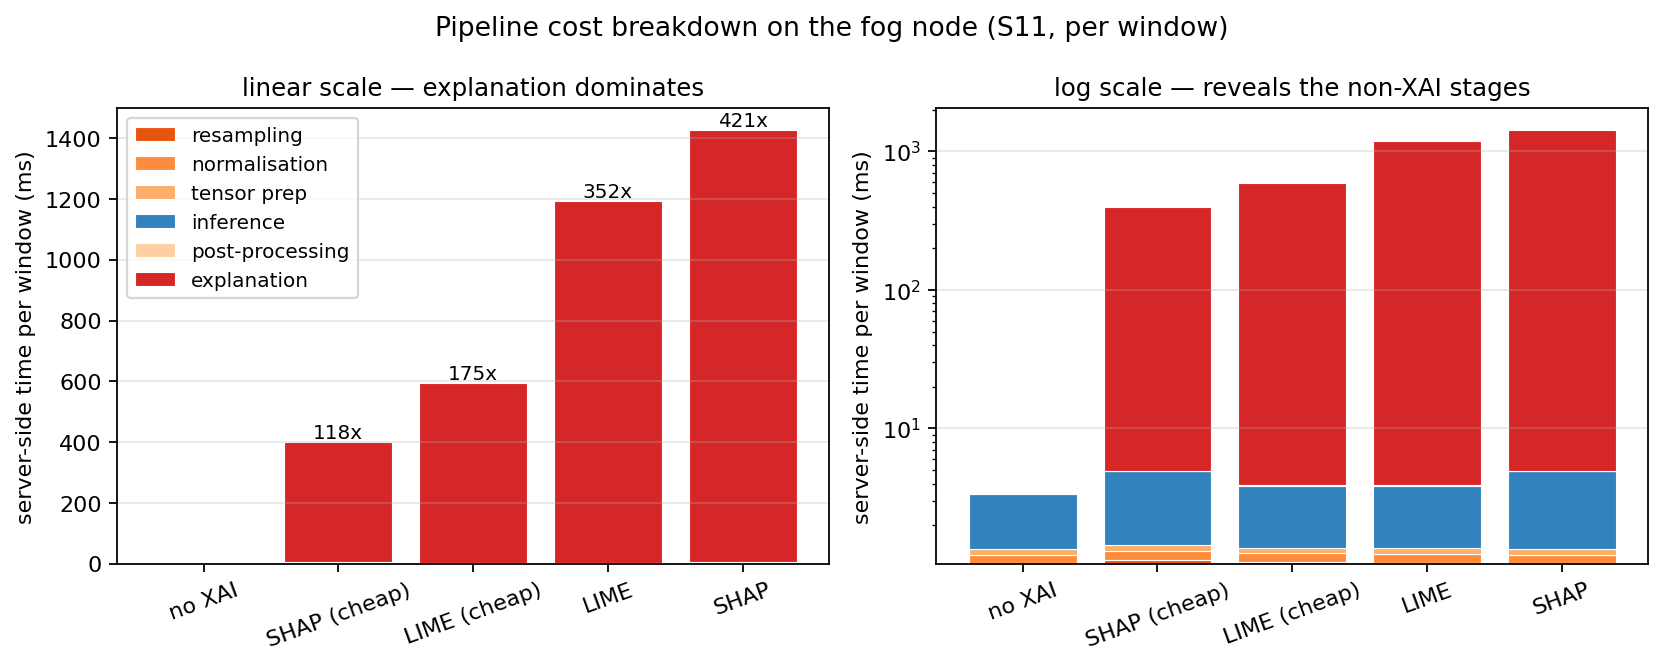
\includegraphics[width=\textwidth]{../results/14_figures/fig1_cost_breakdown.png}
\caption{\textbf{Maliyet dökümü.} Sol panel doğrusal ölçekte: açıklama (kırmızı)
bütün grafiği kaplıyor, diğer aşamalar görünmüyor bile. Sağ panel logaritmik
ölçekte: aynı veri, ama artık yeniden örnekleme (turuncu) ve çıkarım (mavi)
seçilebiliyor. Çubukların üstündeki ``118x'' gibi etiketler, o yapılandırmanın
toplam sunucu hesabının açıklayıcısız tabana (3{,}39\ms) oranıdır.
\emph{Bu şekil tek başına raporun ana bulgusunu taşır.}}
\end{figure}

\begin{figure}[htbp]
\centering
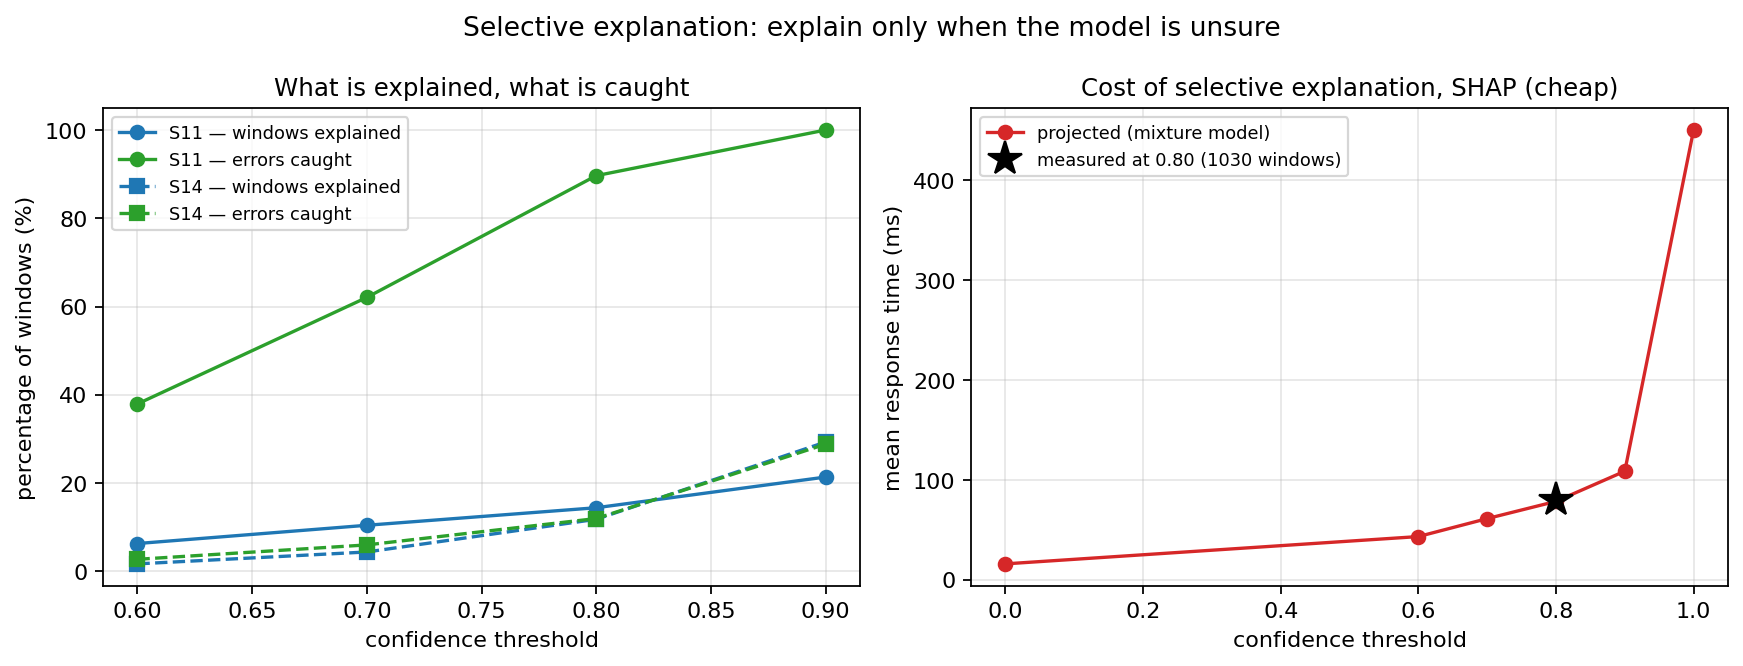
\includegraphics[width=\textwidth]{../results/14_figures/fig2_selective.png}
\caption{\textbf{Seçici açıklama.} Sol panel: eşik yükseldikçe (yatay eksen)
açıklanan pencere oranı (mavi) yavaş, yakalanan hata oranı (yeşil) hızlı
artıyor --- S11'de (düz çizgi) 0{,}80 eşiğinde \%14 pencereyle hataların
\%90'ı yakalanıyor. S14'te (kesikli) aynı eğri çok daha düşük: kalibrasyon
bozuk olduğu için hata yakalama \%12'de kalıyor. Sağ panel: eşiğe karşı
ortalama yanıt süresi. Kırmızı eğri karışım modelinin \emph{projeksiyonu},
siyah yıldız \textbf{1030 pencerelik gerçek ölçüm} --- ikisi üst üste düşüyor.}
\end{figure}

\begin{figure}[htbp]
\centering
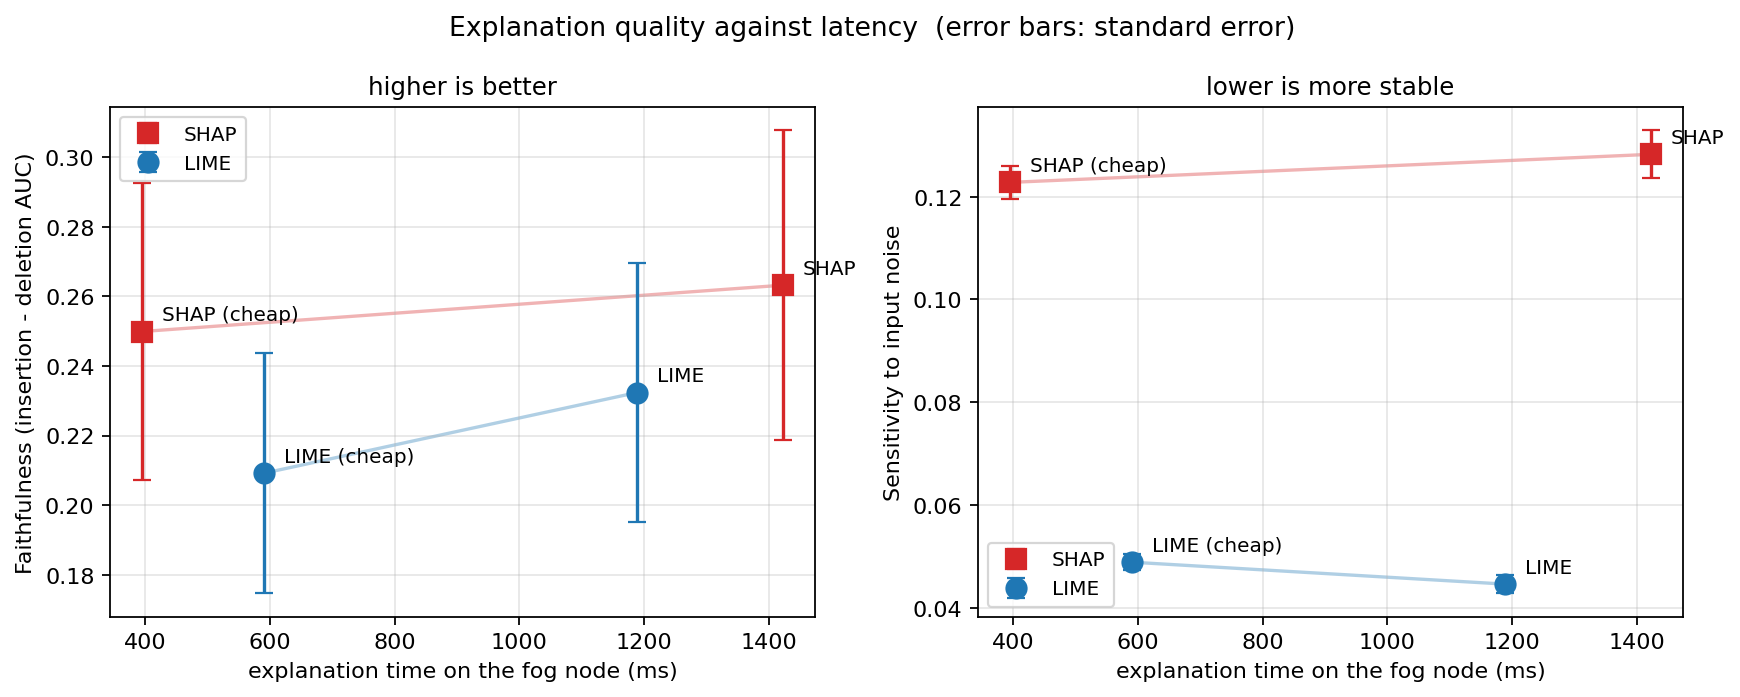
\includegraphics[width=\textwidth]{../results/14_figures/fig3_pareto.png}
\caption{\textbf{Kalite--gecikme dengesi.} Sol panel faithfulness: dört noktanın
hata çubukları \emph{örtüşüyor}, yani sadakat farkı yok. Sağ panel sensitivity:
LIME (mavi, altta) ile SHAP (kırmızı, üstte) arasında açık ve hata payının
çok üstünde bir ayrım var. \emph{Karar faithfulness'a göre değil,
kararlılık ve maliyete göre verilmeli.}}
\end{figure}

\begin{figure}[htbp]
\centering
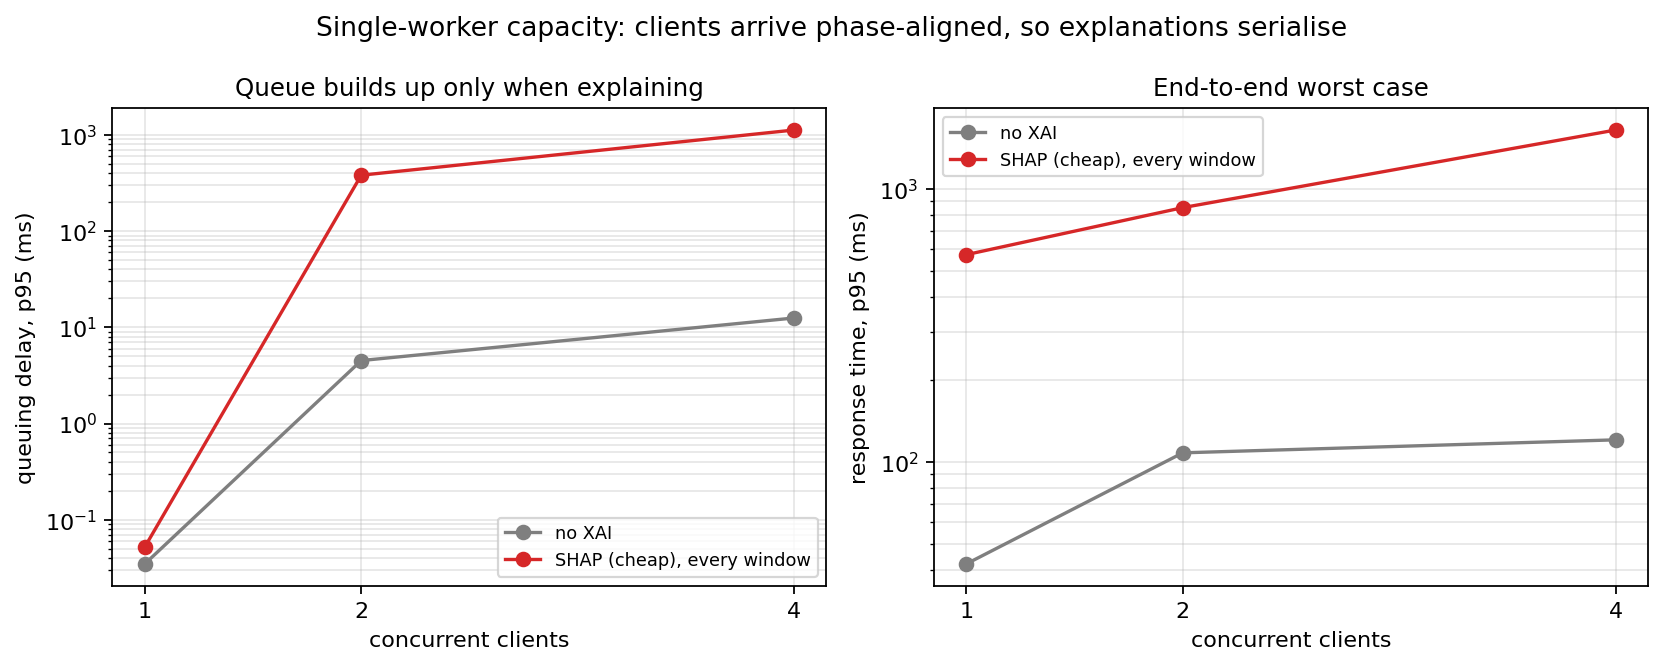
\includegraphics[width=\textwidth]{../results/14_figures/fig4_capacity.png}
\caption{\textbf{Yük altında kapasite} (her iki eksen logaritmik). Sol panel
kuyruk gecikmesi p95: açıklama kapalıyken (gri) 4 istemcide 12{,}5\ms{}'de
kalıyor, açıkken (kırmızı) 1125\ms'ye fırlıyor --- iki büyüklük mertebesi fark.
Sağ panel aynı etkinin uçtan uca yansıması. Eğrilerin doğrusal (log-log'da)
olması $(N-1)\times$açıklama modelini doğruluyor.}
\end{figure}

\begin{figure}[htbp]
\centering
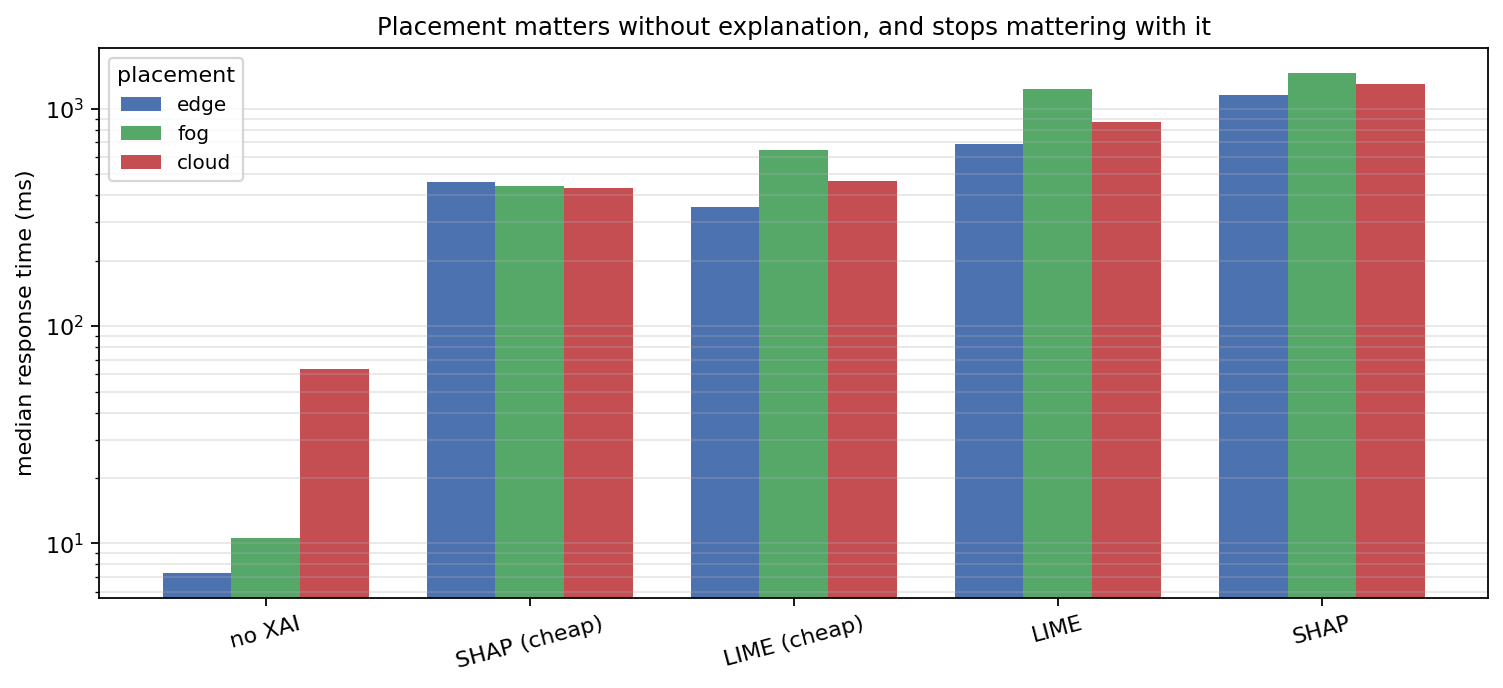
\includegraphics[width=\textwidth]{../results/14_figures/fig5_placement.png}
\caption{\textbf{Yerleşim kararı} (dikey eksen logaritmik). En soldaki grupta
(``no XAI'') üç çubuk arasında büyük fark var: uç 7\ms, sis 11\ms, bulut 64\ms.
Sağa doğru gidildikçe, yani açıklama pahalılaştıkça, üç çubuk birbirine
yaklaşıyor ve en sağdaki grupta (``SHAP'') neredeyse eşitleniyor.
\emph{Yerleşim kararı, açıklama yükü altında anlamını yitiriyor.}}
\end{figure}

\begin{figure}[htbp]
\centering
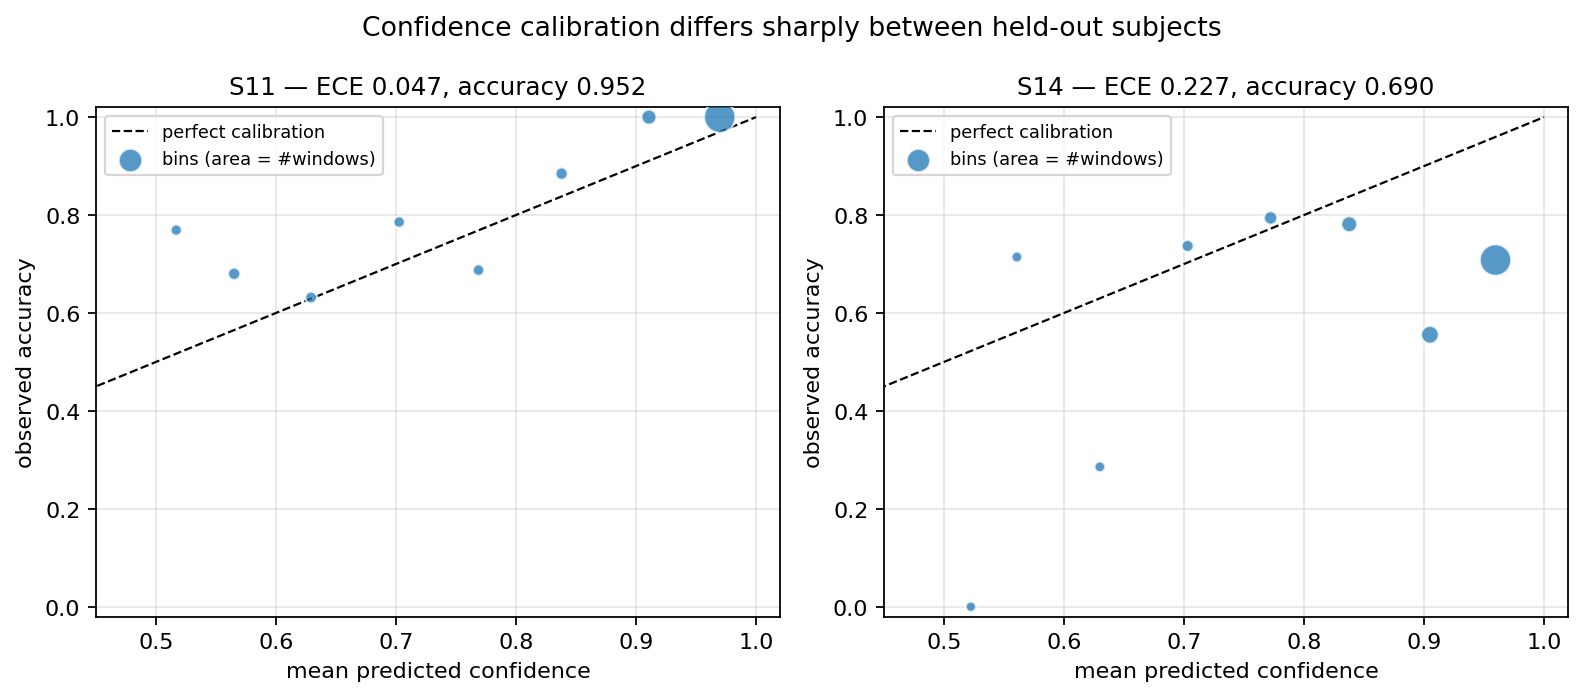
\includegraphics[width=\textwidth]{../results/14_figures/fig6_calibration.png}
\caption{\textbf{Güven kalibrasyonu.} Kesikli köşegen mükemmel kalibrasyonu
gösterir; baloncuk alanı o kutudaki pencere sayısıdır. S11 (sol) noktaları
köşegenin üstünde veya yakınında --- model gerektiği kadar emin. S14 (sağ)
en büyük baloncuk köşegenin \emph{altında}: model \%96 güvenle konuşuyor ama
\%71 haklı. İkisinin ortalama güveni aynı (0{,}909); fark tamamen doğrulukta.}
\end{figure}

\begin{figure}[htbp]
\centering
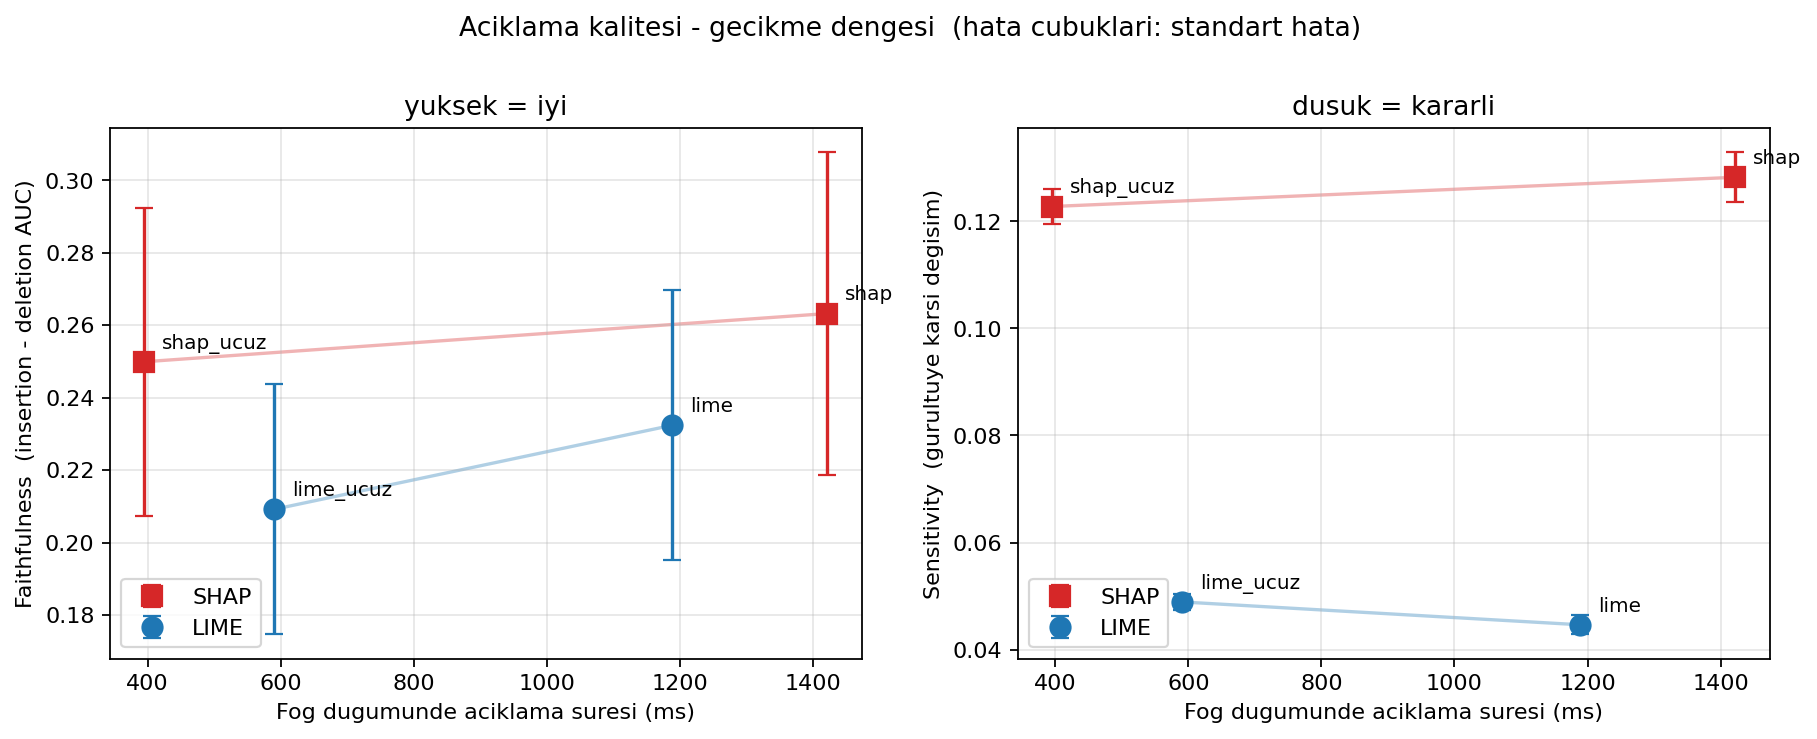
\includegraphics[width=0.95\textwidth]{../results/11_pareto/pareto_c5.png}
\caption{\textbf{Pareto (ayrı üretim).} Şekil 3 ile aynı veriyi gösterir;
\dosya{tools/pareto.py} tarafından üretilen bağımsız sürümüdür.}
\end{figure}

\clearpage

%=======================================================================
\chapter{Donanım Fizibilitesi: Model Bir Mikrodenetleyicide Çalışır mı?}
%=======================================================================

\kod{tools/mcu\_feasibility.py} modelin bir MCU'da çalışıp çalışmayacağını
\emph{donanım olmadan} hesaplar: katman katman parametre, aktivasyon belleği,
tepe RAM ihtiyacı ve MAC sayısı.

\begin{table}[H]
\centering\small
\begin{tabular}{@{}lrrrr@{}}
\toprule
\textbf{Katman} & \textbf{Şekil} & \textbf{Parametre} & \textbf{MAC} & \textbf{Aktivasyon} \\
\midrule
giriş  & 14$\times$640  & 0      & 0          & 8\,960 \\
conv1  & 32$\times$640  & 4\,064 & 2\,580\,480 & 20\,480 \\
bn1    & 32$\times$640  & 64     & 20\,480    & 20\,480 \\
pool1  & 32$\times$320  & 0      & 10\,240    & 10\,240 \\
conv2  & 128$\times$320 & 36\,992 & 11\,796\,480 & 40\,960 \\
bn2    & 128$\times$320 & 256    & 40\,960    & \textbf{40\,960} \\
pool2  & 128$\times$160 & 0      & 20\,480    & 20\,480 \\
gap    & 128            & 0      & 20\,480    & 128 \\
fc1    & 64             & 8\,256 & 8\,192     & 64 \\
bn\_fc & 64             & 128    & 64         & 64 \\
fc2    & 2              & 130    & 128        & 2 \\
\midrule
\textbf{TOPLAM} & & \textbf{49\,890} & \textbf{14\,497\,984} & \\
\bottomrule
\end{tabular}
\caption{Katman katman döküm. Tepe aktivasyon \textbf{81\,920 eleman}
(\kod{bn2} katmanında) --- ikinci evrişim bloğu 128 kanal $\times$ 320 uzunluk
ürettiği için darboğaz orada.}
\end{table}

\begin{table}[H]
\centering\small
\begin{tabular}{@{}lrrr@{}}
\toprule
\textbf{Veri tipi} & \textbf{Ağırlık (Flash)} & \textbf{Tepe RAM} & \textbf{Giriş tamponu} \\
\midrule
float32 & 194{,}9 KB & 320{,}0 KB & 35{,}0 KB \\
float16 & 97{,}4 KB  & 160{,}0 KB & 17{,}5 KB \\
int8    & 48{,}7 KB  & 80{,}0 KB  & 8{,}8 KB \\
\bottomrule
\end{tabular}
\hspace{0.4cm}
\begin{tabular}{@{}lrrcc@{}}
\toprule
\textbf{STM32} & \textbf{RAM} & \textbf{Flash} & \textbf{fp32} & \textbf{int8} \\
\midrule
F103 (M3)  & 20 KB   & 128 KB  & sığmaz & sığmaz \\
F407 (M4)  & 192 KB  & 1 MB    & sığmaz & \textbf{sığar} \\
F746 (M7)  & 320 KB  & 1 MB    & sığmaz & \textbf{sığar} \\
H743 (M7)  & 1 MB    & 2 MB    & \textbf{sığar} & \textbf{sığar} \\
U575 (M33) & 786 KB  & 2 MB    & \textbf{sığar} & \textbf{sığar} \\
\bottomrule
\end{tabular}
\caption{Bellek ihtiyacı ve STM32 ailelerine göre durum. Flash'ın \%80'i,
RAM'in \%80'i sınırı alındı; kalanı program kodu, yığın ve tampon için.}
\end{table}

\begin{table}[H]
\centering\small
\begin{tabular}{@{}lrrr@{}}
\toprule
\textbf{Donanım} & \textbf{MAC/çevrim} & \textbf{tahmini süre} & \textbf{bütçe kullanımı} \\
\midrule
Cortex-M4 @168 MHz, float32 (CMSIS)   & 0{,}3 & 287{,}7\ms & \%5{,}8 \\
Cortex-M7 @480 MHz, float32 (CMSIS)   & 0{,}8 & 37{,}8\ms  & \%0{,}8 \\
Cortex-M7 @480 MHz, int8 (CMSIS-NN)   & 2{,}5 & 12{,}1\ms  & \%0{,}2 \\
\bottomrule
\end{tabular}
\caption{Hız tahmini. Bütçe 5000\ms{} (hop süresi).}
\end{table}

\begin{bulgu}[Hız sorun değil, bellek sorun]
En yavaş senaryo bile hop bütçesinin yirmide birini kullanıyor. MCU'da darboğaz
kesinlikle \textbf{bellek}tir; int8 nicemleme F407/F746 için zorunludur.
\end{bulgu}

\begin{uyari}[Bu analiz kâğıt üstündedir]
Cihaza indirmek için gereken iş: (1) ONNX'e aktarım + STM32Cube.AI ile C kodu,
(2) int8 nicemleme ve doğruluk kaybının ölçümü, (3) ön işlemenin portu
(700\,Hz$\rightarrow$64\,Hz ve nedensel z-score), (4) cihaz üstü ölçüm (DWT
çevrim sayacı, UART raporu), (5) veri beslemesi (SD kart replay ya da UART).
Bu birkaç haftalık bir iştir ve donanım gerektirir.

\textbf{Mimarideki yeri.} STM32 bir mikrodenetleyicidir, işletim sistemi
çalıştırmaz; sis taksonomisinde Raspberry Pi'nin yerini \emph{alamaz}. Ama daha
ilginç bir şeyin yerini alabilir: \textbf{ağın tamamının}. Çıkarım giyilebilir
cihazın içinde yapılırsa uç/sis/bulut seçimi sorunu ortadan kalkar.
\emph{Not:} bu, açıklamayı cihaza taşımaz --- bu raporun ana bulgusu göz önüne
alındığında, XAI'yi bir MCU'ya sığdırmak ayrı ve çok daha zor bir problemdir.
\end{uyari}

%=======================================================================
\chapter{Bitirme Projesinden Gelen Sonuçlar}
\label{sec:bitirme}
%=======================================================================

Depodaki iki Jupyter defteri bitirme projesine aittir ve \textbf{farklı bir
model, farklı bir normalizasyon uzayı ve farklı bir LIME uygulaması}
kullanır. Buradaki sayılar bu raporun geri kalanıyla \emph{karşılaştırılamaz};
arka plan olarak verilmiştir.

\section{\dosya{Transformer.ipynb} --- TranSenseFusers}

\textbf{Mimari.} Temporal CNN + 8 başlı çapraz dikkat (attention dim 64),
14 kanal $\times$ 7000 örnek (10\,s @ 700\,Hz), stride 3500 (\%50 örtüşme),
focal loss ($\alpha$=0{,}75, $\gamma$=2), Adam lr=1e-3, patience 25, seed 42.

\textbf{Protokol.} \kod{TEST\_SUBJECT = 'S3'}, \kod{VAL\_SUBJECT = 'S16'},
kalan 13 denek eğitim. 27.\ epoch'ta erken durdu.

\begin{table}[H]
\centering\small
\begin{tabular}{@{}lrrrr@{}}
\toprule
& \textbf{kesinlik} & \textbf{duyarlılık} & \textbf{F1} & \textbf{n} \\
\midrule
Stres değil & 0{,}9046 & 0{,}9913 & 0{,}9459 & 459 \\
Stres       & 0{,}9518 & \textbf{0{,}6220} & 0{,}7524 & 127 \\
\midrule
doğruluk    & \multicolumn{3}{r}{\textbf{0{,}9113}} & 586 \\
makro ort.  & 0{,}9282 & 0{,}8067 & 0{,}8492 & \\
ağırlıklı   & 0{,}9148 & 0{,}9113 & \textbf{0{,}9040} & \\
\bottomrule
\end{tabular}
\caption{TranSenseFusers, S3 test sonucu. Doğrulama F1'i 1{,}0000 (S16).}
\end{table}

\begin{uyari}
\%91{,}13'lük doğruluk büyük ölçüde \emph{stres-olmayan} sınıftan geliyor:
stres duyarlılığı yalnızca 0{,}6220, yani gerçek streslerin \%38'i kaçırılıyor.
Bu, ``en iyi model'' iddiasını tek başına doğruluk üzerinden kurmanın neden
yanıltıcı olduğunun bir örneğidir.
\end{uyari}

\section{\dosya{XAİ\_metric\_transensefusıon.ipynb} --- offline XAI kalitesi}

\textbf{Kurulum.} TranSenseFusers modeli, 100 örnek (50 stres + 50
stres-olmayan), üç yöntem: SHAP, LIME ve Integrated Gradients.
LIME 700 örneğe indirgenip sonra geri yükseltilmiş.

\begin{table}[H]
\centering\small
\begin{tabular}{@{}lrrrrr@{}}
\toprule
\textbf{Yöntem} & \textbf{Ins-AUC} $\uparrow$ & \textbf{Del-AUC} $\downarrow$ & \textbf{Monotonic} $\downarrow$ & \textbf{Sensitivity} $\downarrow$ & \textbf{Gini} \\
\midrule
SHAP & 0{,}4048 & 0{,}2613 & \textbf{0{,}4047} & \textbf{0{,}0038} & 0{,}6150 \\
LIME & 0{,}4282 & 0{,}2153 & 0{,}5079 & 0{,}0116 & \textbf{0{,}9949} \\
IG   & \textbf{0{,}4402} & \textbf{0{,}2055} & 0{,}5300 & 0{,}0053 & 0{,}6127 \\
\bottomrule
\end{tabular}
\caption{Bitirme projesinin XAI kalite tablosu. Süre ölçülmemiştir.}
\end{table}

\begin{uyari}[Bu tablo bu raporun tablolarıyla karşılaştırılamaz --- dört sebep]
\begin{enumerate}[nosep,leftmargin=1.4em]
\item \textbf{Farklı model} (1{,}86M parametreli transformer vs 49{,}9K CNN).
\item \textbf{Farklı normalizasyon uzayı} (denek bazlı/sızıntılı vs nedensel).
\item \textbf{Farklı LIME uygulaması} (standart \kod{lime} paketi + downsampling
vs bölge tabanlı özel uygulama).
\item \textbf{Monotonicity tanımı ters!} Orada ``düşük iyi'' (ihlal sayısı),
burada ``yüksek iyi'' (azalmayan adım oranı). Aynı isim, farklı şey.
\end{enumerate}
Ayrıca sensitivity ölçeği yaklaşık 10 kat farklı (0{,}004--0{,}012 vs
0{,}045--0{,}128). İki tabloyu yan yana koymak, hakemi ``hangisi doğru''
sorusuna davet eder. Makalede bitirme XAI tablosunun \textbf{yer almaması}
öneriliyor; tek cümlelik atıf yeterli.
\end{uyari}

\textbf{Ölçülen süre bilgisi (defter çıktısından).} 100 örnek için: SHAP
$\approx$0{,}6\,s (177 örnek/s), LIME 2\,dk 37\,s (1{,}57\,s/örnek), IG 33\,s
(3{,}07 örnek/s) --- GPU'da. Bu, bu raporun ana bulgusuyla \emph{niteliksel
olarak} uyumludur: açıklama, çıkarımdan kat kat pahalıdır.

%=======================================================================
\chapter{Geçersiz Sayılan Ölçümler ve Nedenleri}
%=======================================================================

\dosya{results/eski\_ve\_hatali/} klasöründeki dosyalar silinmedi: bir ölçümün
neden geçersiz olduğunu gösteren kayıt da bir kanıttır. ``Neden bunu
kullanmıyoruz'' sorusu makale yazarken ve hakem cevabında tekrar tekrar
karşına çıkacak.

\section{Saat kayması düzeltilmeden önceki sis koşusu}

\dosya{fog\_fog\_1user.json}: \textbf{latency medyanı $-$8{,}75\ms}. Paket
gönderilmeden önce varamayacağı için bu değer fiziksel olarak imkânsızdır.

\textbf{Neden.} Saat farkı yalnızca bağlantı başında bir kez ölçülüyordu. İki
makinenin kristali aynı hızda tiklemediği için fark zamanla kaydı; 87 dakikalık
bu koşuda kayma onlarca milisaniyeye ulaştı.

\textbf{Düzeltme.} Saat farkı artık 60 saniyede bir yeniden ölçülüyor ve her
paketin latency'si iki ölçüm arasında doğrusal ara değerle düzeltiliyor
(\kod{--clock-resync-s}).

\textbf{Kısmen geçerli.} Aynı saatten ölçülen metrikler etkilenmedi: execution
3{,}62\ms, response 8{,}35\ms, 187 kbps, doğruluk \%95{,}2, stres F1 0{,}881.

\section{Sızıntılı normalizasyonla ölçülen XAI taramaları}

\dosya{xai\_sweep\_lime.csv}, \dosya{xai\_sweep\_shap.csv} ve bunlardan
türetilen karşılaştırma. Üç sorun:

\begin{enumerate}[leftmargin=1.5em]
\item \textbf{Yanlış girdi uzayı.} Pencereler deneğin \emph{tüm} kaydının
istatistiğiyle normalize ediliyordu --- geleceğe sızmak. İki uzay ölçüldü:
bağıl L2 farkı 0{,}787 (S11) ve 0{,}773 (S2), standart sapma 1{,}00'e karşı
1{,}25. XAI, dağıtımda görmeyeceği bir girdi dağılımı üzerinde ölçülmüş oldu.

\item \textbf{SHAP kendi gürültüsünü metriğe karıştırdı.} SHAP'ın
\kod{GradientExplainer}'ı her çağrıda rastgele örnekleme yapıyor, seed ise
sabit değildi. Seed sabitlendikten sonra sensitivity 0{,}139'dan
\textbf{0{,}075}'e düştü --- yani ölçülen girdi duyarlılığının neredeyse yarısı, yöntemin
kendi gürültüsüymüş.

\item \textbf{Isınma yok.} Ölçüm döngüsü ilk pencereden başlıyordu.
\end{enumerate}

\textbf{Yine de bir işe yarıyorlar:} iki uzay yan yana konunca sızıntılı ölçümün
XAI'yi olduğundan iyi gösterdiği görülüyor (LIME faithfulness 0{,}2476
$\rightarrow$ 0{,}2333, sensitivity 0{,}0174 $\rightarrow$ 0{,}0264). Makalede
\emph{metodolojik bir not} olarak kullanılabilir --- sonuç olarak değil, karşı
örnek olarak.

\section{\kod{prepared} yol dönemi streaming sonuçları}

Altı dosya. İki sorun: (1) sinyal replay başlamadan 64\,Hz'e indirilmişti, yani
yeniden örnekleme maliyeti ölçüm dışındaydı (toplamın \%29'u); (2) çoğunluk
etiketi geçersiz olan pencereler tamamen atlanıyordu, bu da normalizasyon
istatistiğinin o pencerelerde hiç güncellenmemesi demekti. Gerçek bir sunucu
etiketi görmediği için böyle bir atlama yapamaz. Düzeltildikten sonra doğruluk
0{,}7674'ten \textbf{0{,}8222}'ye çıktı.

\begin{uyari}
\dosya{README.md}'nin ``Ölçülen sonuçlar (S11 + S14, tick=500ms, 1175 pencere)''
tablosundaki sayılar (preprocessing 0{,}189\ms, inference 1{,}15\ms, toplam
1{,}27\ms) \textbf{bu eski koşulardan geliyor} ve güncel değildir. Makaleye
\kod{native} yolun sayıları girmeli.
\end{uyari}

\section{Duman testleri}

\dosya{fog\_statstest.json}, \dosya{deployments\_selftest.json},
\dosya{cloud\_duman\_testi.json}: kodun çalıştığını doğrulama koşuları, ölçüm
değil. \kod{realtime} kapalı olduğu için queuing, jitter ve bandwidth gerçek
yükü yansıtmaz; koşu uzunlukları da rapor için yetersiz.

%=======================================================================
\chapter{Tespit Edilen Tutarsızlıklar}
\label{sec:tutarsizlik}
%=======================================================================

Bu rapor hazırlanırken, \dosya{results/README.md} ile ham JSON/CSV dosyaları
karşılaştırıldı. Aşağıdaki farklar bulundu. \textbf{Hepsinde JSON/CSV
dosyaları esas alınmıştır}, çünkü onlar ölçümün kendisidir.

\begin{longtable}{@{}p{3.2cm}p{5.2cm}p{5.6cm}@{}}
\toprule
\textbf{Yer} & \textbf{\dosya{results/README.md} ne diyor} & \textbf{Dosya ne diyor} \\
\midrule
\endfirsthead
\toprule
\textbf{Yer} & \textbf{README ne diyor} & \textbf{Dosya ne diyor} \\
\midrule
\endhead
\dosya{02\_benchmark/\newline benchmark\_xai\_cpu} &
``LIME 250 örnek p50 490\ms'' &
Dosyada 250 örneklik bir kayıt \textbf{yok}. İki kayıt var: 500/20/0{,}5 (p50 710\ms) ve 500/\textbf{5}/0{,}25 (p50 678\ms). \\
\addlinespace
\dosya{05\_yerlesim} &
uç latency 0{,}81, execution 6{,}19, response 7{,}44\ms; sis latency 3{,}69, execution 3{,}61, response 9{,}97\ms &
uç 0{,}928 / 6{,}344 / 7{,}880; sis 4{,}910 / 3{,}372 / 10{,}151 (üç tekrarın medyanlarının medyanı). \\
\addlinespace
\dosya{01\_streaming} &
``1175 pencere'' &
\kod{n\_windows} = 2123 ölçülen pencere; etiketli pencere 1198. \\
\addlinespace
\dosya{04\_fog} tablosu &
``execution 3{,}5\ms{}'' (none) &
\kod{execution.mean\_ms} = 3{,}586; \kod{median\_ms} = 3{,}530. İkisi de doğru, ama hangisi olduğu yazılmalı. \\
\addlinespace
\dosya{09\_secici\_xai} &
``hiç açıklama ort.\ response 15{,}9\ms{}'' &
Doğru, ama bu \dosya{04\_fog/fog\_xai\_none}'un \emph{ortalaması}; aynı README başka yerde aynı koşu için medyanı (10{,}6) veriyor. Karşılaştırma tablolarında ikisi karışmamalı. \\
\bottomrule
\caption{Bulunan tutarsızlıklar. Hiçbiri sonuçları değiştirmiyor, ama makaleye
sayı taşınırken \textbf{doğrudan JSON'dan okunmalı}.}
\end{longtable}

\begin{bulgu}[Öneri]
\kod{tools/paper\_tables.py} yazılmalı: Bölüm~\ref{sec:fog} ve
\ref{sec:secici}'deki tabloları JSON'dan LaTeX \kod{tabular} olarak üretsin ve
makaleye \kod{\textbackslash input\{\}} ile girsin. Elle sayı kopyalandığı
sürece bu tür kaymalar tekrar olur.
\end{bulgu}

%=======================================================================
\chapter{Sentez: Bütün Sonuçlar Bir Arada}
%=======================================================================

\section{Sistemin tam maliyet resmi}

\begin{table}[H]
\centering\small
\begin{tabular}{@{}lrl@{}}
\toprule
\textbf{Bileşen} & \textbf{Süre} & \textbf{Payı} \\
\midrule
\multicolumn{3}{@{}l}{\emph{Veri toplama (hesap değil)}} \\
pencere uzunluğu & 10\,000\ms & --- \\
güncelleme aralığı (hop) & 5\,000\ms & \textbf{bütçe} \\
\midrule
\multicolumn{3}{@{}l}{\emph{Sunucu hesabı, açıklama kapalı (sis düğümü)}} \\
resampling      & 1{,}05\ms & \%31 \\
preprocessing   & 0{,}17\ms & \%5 \\
tensor\_prep    & 0{,}11\ms & \%3 \\
inference       & 2{,}01\ms & \%59 \\
postprocessing  & 0{,}05\ms & \%1 \\
\textbf{toplam} & \textbf{3{,}39\ms} & \textbf{bütçenin \%0{,}07'si} \\
\midrule
\multicolumn{3}{@{}l}{\emph{Açıklama (her pencerede)}} \\
\kod{shap\_cheap} & 395\ms & bütçenin \%7{,}9'u \\
\kod{lime\_cheap} & 590\ms & bütçenin \%11{,}8'i \\
\kod{lime}        & 1189\ms & bütçenin \%23{,}8'i \\
\kod{shap}        & 1422\ms & bütçenin \%28{,}4'ü \\
\midrule
\multicolumn{3}{@{}l}{\emph{Ağ (tek yön)}} \\
uç (loopback)   & $\approx$1\ms & \\
sis (Wi-Fi)     & 4--5\ms & \\
bulut (internet)& 40--60\ms & \\
\bottomrule
\end{tabular}
\caption{Uçtan uca maliyet resmi. \textbf{En büyük tek kalem, bütün ağ ve hesap
bileşenlerinin toplamından yüzlerce kat büyük olan açıklamadır.}}
\end{table}

\section{Neden tek kullanıcıda bile önemli}

Tek kullanıcıda 1422\ms'lik en pahalı açıklama bile 5000\ms{} bütçesine sığıyor
(\%28), dolayısıyla ``sorun yok'' denebilirmiş gibi görünür. Üç sebeple sorun
vardır:

\begin{enumerate}[leftmargin=1.5em]
\item \textbf{Çok kullanıcıda sığmıyor.} 4 istemcide kuyruk p95 1125\ms;
kapasite hep-açıkla durumunda 12 istemciye düşüyor.
\item \textbf{Zayıf donanımda sığmıyor.} Referans çalışmanın Raspberry Pi 4
worker'ında execution 34{,}7\ms, bu çalışmada 3{,}6\ms{} --- yaklaşık
\textbf{10 kat} fark. Aynı oran açıklamaya uygulanırsa \kod{shap\_cheap} bir
Pi 4'te \textbf{$\approx$4 saniye} eder ve 5 saniyelik bütçeyi neredeyse
doldurur.
\item \textbf{Kullanıcı deneyimi.} 1456\ms'lik bir yanıt, 10{,}6\ms'lik bir
yanıtın yanında ``sistem takıldı'' hissi verir.
\end{enumerate}

\section{Referans makale ile karşılaştırma}

Erzurumluoğlu ve ark., ICACT 2025; DREAMER veri setiyle sis mimarisinde duygu
tanıma. Worker düğümü Raspberry Pi 4.

\begin{table}[H]
\centering\small
\begin{tabular}{@{}lrrl@{}}
\toprule
\textbf{Metrik} & \textbf{Makale (worker)} & \textbf{Bu çalışma} & \textbf{Karşılaştırılabilir mi?} \\
\midrule
latency        & 4{,}7\ms  & 0{,}81\ms (loopback) & hayır --- farklı ağ \\
queuing delay  & $<$1\ms   & 0{,}045\ms & hayır \\
execution time & 34{,}7\ms & 7{,}18\ms  & hayır --- Pi 4 vs masaüstü \\
response time  & 43{,}3\ms & 8{,}82\ms  & hayır \\
jitter         & 17{,}4\ms & 3{,}53\ms  & hayır \\
\textbf{bandwidth} & \textbf{374 kbps} & \textbf{187 kbps} & \textbf{evet} \\
\bottomrule
\end{tabular}
\caption{Yalnızca bant genişliği doğrudan karşılaştırılabilir.}
\end{table}

\begin{bulgu}[Anlamlı olan tek karşılaştırma]
Onlar 3 saniyelik pencereden 24 öznitelik çıkarıp gönderiyor, biz 10 saniyelik
pencerenin \textbf{ham sinyalini} gönderiyoruz --- buna rağmen \textbf{yarısı
kadar} veri geçiyor.

Asıl fark mimari: onların sisteminde öznitelik çıkarımı hesabın çoğunu
oluşturuyor, bizde ham sinyal doğrudan modele giriyor ve hesap çok daha ucuz.
Buna karşılık bizim uçtan uca gecikmemizi \emph{hesap değil pencere uzunluğu}
belirliyor: 10 saniyelik pencere, 8{,}8\ms{} yanıt süresinin bin katından fazla.

\textbf{Broker neden gerekmiyor.} Onların mimarisinde broker, istekleri en az
yüklü worker'a dağıtan bir yönlendiricidir. Tek worker varken dağıtacak bir şey
yoktur. Kendi sonuçlarında da broker ile worker sayıları neredeyse aynı çıkmış
(43{,}9'a karşı 43{,}3\ms).
\end{bulgu}

%=======================================================================
\chapter{Sınırlılıklar}
%=======================================================================

\begin{enumerate}[leftmargin=1.6em,itemsep=0.5em]

\item \textbf{İki tutulmuş denek (n=2).} Kalibrasyon bulgusu ve ``denek
bağımlı'' sonucu yalnızca S11 ve S14 üzerine kurulu. Bu bir genelleme değil,
bir gözlemdir.

\item \textbf{Sis düğümü bir masaüstü, Raspberry Pi değil.} Ölçülen şey
\emph{dağıtık yerleşim}dir, \emph{kaynak kısıtlı sis düğümü} değil. Ölçüldü ki
tek çekirdeğe kilitlemek bu iş yükünde hiçbir şey değiştirmiyor: süreç zaten
tek iplik ve bir çekirdeği aşmıyor (tepe CPU \%105--111). Bağlayıcı olan tek
yöntem kesirli CPU kotasıdır (Docker \kod{--cpus=0.1}).

\item \textbf{Yazılım yığını yerleşimler arasında farklı.} Uç: Python 3.11 /
PyTorch 2.8. Sis: Python 3.14 / PyTorch 2.14. Bulut: Docker python:3.11 /
PyTorch 2.14. Bu, 07\_edge\_xai ile 04\_fog arasındaki tutarsız sıralamanın
sebebidir. Kapatmak için sis düğümünü Docker'la yeniden koşmak yeterli
($\approx$25 dk).

\item \textbf{Kuyruk ölçümü bir üst sınırdır.} İstemciler eşzamanlı başlatıldığı
için faz hizalı kalıyor. Gerçek dağıtımda rastgele fazlarda başlarlar.

\item \textbf{Sis XAI koşuları 44 pencere, tek tekrar.} Ortalama karşılaştırması
için yeterli; p95/p99 yalnızca 1030 pencerelik seçici koşudan alınmalı.

\item \textbf{Kullanıcı çalışması yok.} Açıklamaların insanlara gerçekten
yardım edip etmediği ölçülmedi. Bu standart bir XAI sınırlılığıdır.

\item \textbf{Tek model, iki açıklayıcı.} Model karmaşıklığı ablasyonu (aynı
mimarinin küçük/büyük varyantları) ve Integrated Gradients kapsam dışı.

\item \textbf{Latency Wi-Fi'da ve internette belirsiz.} Tek yönlü gecikmenin
hata payı Wi-Fi'da $\pm$1--1{,}7\ms, internette $\pm$25--51\ms. Execution,
queuing (sunucu saati), response ve jitter (istemci saati) bundan etkilenmez.

\item \textbf{Emülasyon, canlı sistem değil.} WESAD kaydından replay yapılıyor.
Bu, referans makalenin de yaptığı şeydir ve yöntemin savunulabilirliği buna
dayanır --- ama ``clinical'' ya da ``live system'' denmemelidir.

\end{enumerate}

%=======================================================================
\chapter{Ekler}
%=======================================================================

\section{Her sayı hangi dosyadan}

{\small
\begin{longtable}{@{}p{6.4cm}p{8.1cm}@{}}
\toprule
\textbf{Sonuç} & \textbf{Kaynak dosya} \\
\midrule
\endfirsthead
\toprule
\textbf{Sonuç} & \textbf{Kaynak dosya} \\
\midrule
\endhead
Aşama bazlı hesaplama profili (tek süreç) & \dosya{01\_streaming/streaming\_summary\_native\_fixed.json} \\
İplik taraması, koşu arası yayılım & \dosya{02\_benchmark/benchmark\_thread\_sweep.json} \\
\kod{prepared} vs \kod{native} & \dosya{02\_benchmark/benchmark\_pipeline\_cmp.json} \\
Açıklayıcıların istemci CPU maliyeti & \dosya{02\_benchmark/benchmark\_xai\_cpu.json} \\
Yedi metrik, loopback & \dosya{03\_loopback/fog\_realtime\_1user.json} \\
Kuyruk metriğinin doğrulanması & \dosya{03\_loopback/fog\_full\_queue.json} \\
\textbf{Ana maliyet tablosu (sis)} & \dosya{04\_fog/fog\_xai\_\{none,shapucuz,
ewline limeucuz,lime,shap\}.json} \\
Uç vs sis (XAI'siz) & \dosya{05\_yerlesim/deployments\_edge\_vs\_fog.json} \\
XAI hiperparametre taraması & \dosya{06\_xai\_tarama/xai\_sweep\_\{lime,shap\}\_causal.csv} \\
Ortak yerleşimde XAI & \dosya{07\_edge\_xai/edge\_xai\_*.json} \\
Kalibrasyon, ECE, eşik tablosu & \dosya{08\_kalibrasyon/calibration\_d1.json} \\
\textbf{Seçici açıklama, ana koşu} & \dosya{09\_secici\_xai/fog\_sel80\_tam.json} \\
Eşik projeksiyonu (48 satır) & \dosya{09\_secici\_xai/selective\_xai\_sweep\_d2.json} \\
Eşiğin tetiklenmediği koşular & \dosya{09\_secici\_xai/kisa\_segment\_sel\{60,80,90\}.json} \\
Çok istemcili yük ve kapasite & \dosya{10\_yuk/fog\_load\_\{none,shapucuz\}\_\{2,4\}.json} \\
Kalite--gecikme Pareto & \dosya{11\_pareto/pareto\_c5.json} \\
Dört kaynaktan aşama derlemesi & \dosya{12\_profil/profile\_table\_b1.json} \\
Bulut yerleşimi & \dosya{13\_bulut/cloud\_\{taban\_3tur,xai\_*,load\_4\}.json} \\
Altı şekil & \dosya{14\_figures/fig\{1..6\}\_*.png} \\
Seçilmiş XAI yapılandırmaları & \dosya{checkpoints/xai\_config.json} \\
SHAP arka plan kümesi & \dosya{checkpoints/shap\_background\_k100\_kmeans.npz} \\
MCU fizibilitesi & \kod{python -m tools.mcu\_feasibility} (kayıtsız) \\
TranSenseFusers başarımı & \dosya{Transformer.ipynb}, hücre 10 \\
Offline XAI kalite tablosu & \dosya{XAİ\_metric\_transensefusıon.ipynb}, hücre 1 \\
\bottomrule
\end{longtable}}

\section{Deneyleri yeniden koşma komutları}

\begin{tcolorbox}[colback=acikGri,colframe=black!30,boxrule=0.6pt,breakable]
\ttfamily\footnotesize
\# 01 --- tek süreçli replay\\
python run\_streaming\_emulation.py --subject S11 S14 --tag native\_fixed\\[0.5em]

\# 02 --- tekrarlı, dönüşümlü ölçüm\\
python benchmark\_runs.py --subject S11 --repeat 4 --threads 1 2 4 --tag thread\_sweep\\
python benchmark\_runs.py --subject S11 --repeat 4 --pipeline prepared native --tag pipeline\_cmp\\[0.5em]

\# 03 --- loopback, yedi metrik\\
python run\_fog\_experiment.py --subject S11 --realtime --tag realtime\_1user\\[0.5em]

\# Sunucuyu ikinci makinede başlat (XAI ile)\\
python -m serving.server --host 0.0.0.0 --port 9099 \textbackslash\\
\hspace*{2em}--xai-method shap\_cheap --xai-threshold 1.0\\[0.5em]

\# 04 --- sis düğümünde XAI (her durum için ayrı)\\
python run\_fog\_experiment.py --server-host 192.168.1.14 --subject S11 \textbackslash\\
\hspace*{2em}--realtime --max-ticks 600 --tag xai\_shapucuz\\[0.5em]

\# 05 --- yerleşim karşılaştırması\\
python compare\_deployments.py --subject S11 --realtime --max-ticks 600 --repeat 3 \textbackslash\\
\hspace*{2em}--deployment edge=local fog=192.168.1.14 --tag edge\_vs\_fog\\[0.5em]

\# 08 --- kalibrasyon\\
python -m tools.calibration --tag d1\\[0.5em]

\# 09 --- seçici XAI (sunucuda --xai-threshold 0.8 ile)\\
python run\_fog\_experiment.py --server-host 192.168.1.14 --subject S11 \textbackslash\\
\hspace*{2em}--realtime --tag sel80\_tam\\
python -m tools.selective\_sweep --tag d2\\[0.5em]

\# 10 --- çok istemcili yük\\
python run\_fog\_experiment.py --server-host 192.168.1.14 --subject S11 S14 \textbackslash\\
\hspace*{2em}--clients 4 --realtime --max-ticks 600 --tag load\_4\\[0.5em]

\# 11, 12, 14 --- türetilmiş çıktılar\\
python -m tools.pareto --tag c5\\
python -m tools.profile\_table\\
python -m tools.figures\\[0.5em]

\# Donanımsız MCU analizi\\
python -m tools.mcu\_feasibility
\end{tcolorbox}

\section{Docker ile sunucuyu dağıtma}

\begin{tcolorbox}[colback=acikGri,colframe=black!30,boxrule=0.6pt]
\ttfamily\footnotesize
\# Sunucu makinesinde\\
WESAD\_XAI\_METHOD=shap\_cheap WESAD\_XAI\_THRESHOLD=0.8 \textbackslash\\
docker compose up -d --build\\
docker compose logs -f stress-server\\[0.5em]
\# Sunucu WESAD verisine İHTİYAÇ DUYMAZ --- veri istemcide kalır.
\end{tcolorbox}

\section{Bu raporu yeniden derleme}

\begin{tcolorbox}[colback=acikGri,colframe=black!30,boxrule=0.6pt]
\ttfamily\footnotesize
cd docs\\
xelatex teknik\_rapor.tex\\
xelatex teknik\_rapor.tex\hspace{2em}\# içindekiler için ikinci geçiş
\end{tcolorbox}

Şekiller, depo kökündeki \dosya{results/14\_figures/} ve
\dosya{results/11\_pareto/} klasörlerinden okunur. Bu şekilleri üreten
betikler yeniden koşulursa rapor da güncel hâllerini alır.

\vspace{1.5em}
\begin{center}
\rule{0.4\textwidth}{0.4pt}
\end{center}

\end{document}
